%\VignetteIndexEntry{gaston package}
%\VignetteDepends{gaston}
%\VignettePackage{gaston}
%\VignetteEngine{knitr::knitr}

\documentclass{article}\usepackage[]{graphicx}\usepackage[]{color}
%% maxwidth is the original width if it is less than linewidth
%% otherwise use linewidth (to make sure the graphics do not exceed the margin)
\makeatletter
\def\maxwidth{ %
  \ifdim\Gin@nat@width>\linewidth
    \linewidth
  \else
    \Gin@nat@width
  \fi
}
\makeatother

\definecolor{fgcolor}{rgb}{0.345, 0.345, 0.345}
\newcommand{\hlnum}[1]{\textcolor[rgb]{0.686,0.059,0.569}{#1}}%
\newcommand{\hlstr}[1]{\textcolor[rgb]{0.192,0.494,0.8}{#1}}%
\newcommand{\hlcom}[1]{\textcolor[rgb]{0.678,0.584,0.686}{\textit{#1}}}%
\newcommand{\hlopt}[1]{\textcolor[rgb]{0,0,0}{#1}}%
\newcommand{\hlstd}[1]{\textcolor[rgb]{0.345,0.345,0.345}{#1}}%
\newcommand{\hlkwa}[1]{\textcolor[rgb]{0.161,0.373,0.58}{\textbf{#1}}}%
\newcommand{\hlkwb}[1]{\textcolor[rgb]{0.69,0.353,0.396}{#1}}%
\newcommand{\hlkwc}[1]{\textcolor[rgb]{0.333,0.667,0.333}{#1}}%
\newcommand{\hlkwd}[1]{\textcolor[rgb]{0.737,0.353,0.396}{\textbf{#1}}}%
\let\hlipl\hlkwb

\usepackage{framed}
\makeatletter
\newenvironment{kframe}{%
 \def\at@end@of@kframe{}%
 \ifinner\ifhmode%
  \def\at@end@of@kframe{\end{minipage}}%
  \begin{minipage}{\columnwidth}%
 \fi\fi%
 \def\FrameCommand##1{\hskip\@totalleftmargin \hskip-\fboxsep
 \colorbox{shadecolor}{##1}\hskip-\fboxsep
     % There is no \\@totalrightmargin, so:
     \hskip-\linewidth \hskip-\@totalleftmargin \hskip\columnwidth}%
 \MakeFramed {\advance\hsize-\width
   \@totalleftmargin\z@ \linewidth\hsize
   \@setminipage}}%
 {\par\unskip\endMakeFramed%
 \at@end@of@kframe}
\makeatother

\definecolor{shadecolor}{rgb}{.97, .97, .97}
\definecolor{messagecolor}{rgb}{0, 0, 0}
\definecolor{warningcolor}{rgb}{1, 0, 1}
\definecolor{errorcolor}{rgb}{1, 0, 0}
\newenvironment{knitrout}{}{} % an empty environment to be redefined in TeX

\usepackage{alltt}
%\usepackage[noae]{Sweave}
\usepackage[top=35mm, bottom=40mm, left=25mm , right=25mm]{geometry}
%\usepackage{moreverb}
\usepackage[utf8]{inputenc}
\usepackage{amsfonts}
\usepackage{amsmath}
\usepackage{etoolbox}

%\setkeys{Gin}{width=0.4\textwidth}
%\SweaveOpts{echo=TRUE, eps=FALSE, pdf=TRUE}

\raggedbottom
\pagestyle{empty}
\parindent0pt
\parskip8pt
\def\thesection{\arabic{section}}
\def\theequation{\arabic{equation}}
\let\epsilon\varepsilon

%<<echo=FALSE>>=
%options(continue=" ", prompt = " ", SweaveHooks=list(fig.mar=function() par(mar=c(5.1,4.1,3.1,2.1))), width=90)
%@


%<<prompton, echo=FALSE>>=
%options(prompt="> ", continue = " ");
%@


%<<promptoff, echo=FALSE>>=
%options(prompt=" ", continue=" ");
%@






\title{{\bfseries Gaston}\\
       {\large Version 1.5.3}}
\author{Hervé Perdry, Claire Dandine-Roulland}


%\DefineVerbatimEnvironment{Sinput}{Verbatim}{}
%\DefineVerbatimEnvironment{Soutput}{Verbatim}{}
%\DefineVerbatimEnvironment{Scode}{Verbatim}{}
%\fvset{listparameters={\setlength{\topsep}{-0.5em}}}
%\renewenvironment{Schunk}{\vspace{\topsep}}{\vspace{\topsep}}
\makeatletter
\preto{\@verbatim}{\topsep=2pt \partopsep=-10pt }
\preto{\alltt}{\topsep=-3pt \partopsep=-10pt }
\makeatother
\IfFileExists{upquote.sty}{\usepackage{upquote}}{}
\begin{document}
\maketitle

%%%%%%%%%%%%%%%%%%%%%%%%%%%%%%%%%%%%%%%%%%%%%%%%%%%%%%%%%%%%%%%%%%%%%%%%%%%%%%%%%%%%%%%%%%%%%%%%%%%%
\section*{Introduction}

  Gaston offers functions for efficient manipulation of 
  large genotype (SNP) matrices, and state-of-the-art implementation of algorithms
  to fit Linear Mixed Models, that can be used to compute heritability 
  estimates or to perform association tests.
  Thanks to the packages \verb!Rcpp!, \verb!RcppParallel!, \verb!RcppEigen!, Gaston
  functions are mainly written in C++. Many are multithreaded.

  For better performances, we recommend to build Gaston with \verb!clang++!.
  To do so, it is sufficient to create in your home directory
  a file \verb!~/.R/Makevars! containing \verb!CXX1X = clang++! 
  or if you use a version of R $>=$ 3.4.0, \verb!CXX11 = clang++!

  In this vignette, we illustrate Gaston using the included data sets \verb!AGT!, \verb!LCT!,
  and \verb!TTN! (see the corresponding manual pages for a description). 
  Gaston also includes some example files in the \verb!extdata! folder. 
  Not all options of the functions are described here, but rather their basic usage.
  The reader is advised to look at the manual pages for details.

  Note that the package name is written \verb!gaston! when dealing with R commands, 
  but Gaston (with a capital) in human language.

\section{Modifying Gaston's behaviour with global options}

\subsection{Number of threads}

  The number of threads used by multithreaded functions can be modified 
  through \verb!RcppParallel!  function \verb!setThreadOptions!.
  It is advised to try several values for the number of threads, as 
  using too many threads might be counterproductive due to an important
  overhead. The default value set by \verb!RcppParallel! is generally
  too high.

  Some functions have a \verb!verbose! argument, which controls the
  function verbosity. To mute all functions at once you can use 
  \verb!options(gaston.verbose = FALSE)!.

\subsection{Basic statistics computations}

  Since version 1.4, the behaviour of all functions that output a
  matrix of genotypes (a bed.matrix, described in the next section)
  can be modified by setting \verb!options(gaston.auto.set.stats = FALSE)!.
  The effects of this option is described in section \ref{stats}
  below. Note that some examples in the manual pages might not work if
  you use this option.

\subsection{Autosomes, gonosomes, mitochondria}

  Since version 1.4.7, some functions take into account wether a SNP 
  is autosomal, X or Y linked, or mitochondrial. The ids of the corresponding
  chromosomes are defined by options \verb!gaston.autosomes!, \verb!gaston.chr.x!,
  \verb!gaston.chr.y!, \verb!gaston.chr.mt!. Default values are \verb!c(1:22, 25)!,
  \verb!23!, \verb!24! and \verb!26!, following to Plink convention (in this
  convention, \verb!25! corresponds to the pseudo-autosomal XY region: we chose
  to include it in the autosomes).

%%%%%%%%%%%%%%%%%%%%%%%%%%%%%%%%%%%%%%%%%%%%%%%%%%%%%%%%%%%%%%%%%%%%%%%%%%%%%%%%%%%%%%%%%%%%%%%%%%%%
\section{Genotype matrices}

  An S4 class for genotype matrices is defined, named \verb!bed.matrix!.
  Each row correspond to an individual, and each column to a SNP. 

\subsection{Reading bed.matrices from files}

  Bed.matrices be read from files using \verb!read.bed.matrix!.
  The function \verb!read.vcf! reads VCF files; it relies on the package \verb!WhopGenome!.

  Gaston includes example files that can be used for illustration:

\begin{knitrout}
\definecolor{shadecolor}{rgb}{0.969, 0.969, 0.969}\color{fgcolor}\begin{kframe}
\begin{alltt}
\hlstd{> }\hlstd{x} \hlkwb{<-} \hlkwd{read.bed.matrix}\hlstd{(} \hlkwd{system.file}\hlstd{(}\hlstr{"extdata"}\hlstd{,} \hlstr{"LCT.bed"}\hlstd{,} \hlkwc{package}\hlstd{=}\hlstr{"gaston"}\hlstd{) )}
\end{alltt}
\begin{verbatim}
Reading /home/rv/R/R-3.4/gaston/extdata/LCT.rds 
Reading /home/rv/R/R-3.4/gaston/extdata/LCT.bed 
\end{verbatim}
\begin{alltt}
\hlstd{> }\hlstd{x}
\end{alltt}
\begin{verbatim}
A bed.matrix with 503 individuals and 607 markers.
snps stats are not set (or incomplete)
ped stats are not set (or incomplete)
\end{verbatim}
\end{kframe}
\end{knitrout}
  
  The folder \verb!extdata/! contains files \verb!LCT.bed!, \verb!LCT.rds!,
  \verb!LCT.bim! and \verb!LCT.fam!. The \verb!.bed!, \verb!.bim! and \verb!.fam! files follow the
  PLINK specifications. The \verb!.rds! file is a R data file; if it is present, the
  \verb!.bim! and \verb!.fam! files are ignored. You can ignore the
  \verb!.rds! file using option \verb!rds = NULL!:

\begin{knitrout}
\definecolor{shadecolor}{rgb}{0.969, 0.969, 0.969}\color{fgcolor}\begin{kframe}
\begin{alltt}
\hlstd{> }\hlstd{x} \hlkwb{<-} \hlkwd{read.bed.matrix}\hlstd{(} \hlkwd{system.file}\hlstd{(}\hlstr{"extdata"}\hlstd{,} \hlstr{"LCT.bed"}\hlstd{,} \hlkwc{package}\hlstd{=}\hlstr{"gaston"}\hlstd{),} \hlkwc{rds} \hlstd{=} \hlkwa{NULL} \hlstd{)}
\end{alltt}
\begin{verbatim}
Reading /home/rv/R/R-3.4/gaston/extdata/LCT.fam 
Reading /home/rv/R/R-3.4/gaston/extdata/LCT.bim 
Reading /home/rv/R/R-3.4/gaston/extdata/LCT.bed 
ped stats and snps stats have been set. 
'p' has been set. 
'mu' and 'sigma' have been set.
\end{verbatim}
\begin{alltt}
\hlstd{> }\hlstd{x}
\end{alltt}
\begin{verbatim}
A bed.matrix with 503 individuals and 607 markers.
snps stats are set
ped stats are set
\end{verbatim}
\end{kframe}
\end{knitrout}

  A bed.matrix can be saved using \verb!write.bed.matrix!.  
  The default behavior is to write \verb!.bed!, \verb!.bim!, \verb!.fam! 
  and \verb!.rds! files; see the manual page for more details.

\subsection{Conversion from and to R objects}

  A numerical matrix \verb!x! containing genotype counts (0, 1, 2 or \verb!NA!) can be 
  transformed in a bed.matrix with \verb!as(x, "bed.matrix")!. The resulting
  object will lack individual and SNP informations (if the rownames and colnames
  of \verb!x! are set, they will be used as SNP and individual ids respectively).

  Conversely, a numerical matrix can be retrieved from a bed.matrix using \verb!as.matrix!. 
  
  The function \verb!as.bed.matrix! allows to provide data frames corresponding to 
  the \verb!.fam! and \verb!.bim! files. They should have colnames \verb!famid!, 
  \verb!id!, \verb!father!, \verb!mother!, \verb!sex!, \verb!pheno!, and \verb!chr!, \verb!id!, 
  \verb!dist!, \verb!pos!, \verb!A1!, \verb!A2! respectively. This function is widely used in
  the examples included in manual pages.

\begin{knitrout}
\definecolor{shadecolor}{rgb}{0.969, 0.969, 0.969}\color{fgcolor}\begin{kframe}
\begin{alltt}
\hlstd{> }\hlkwd{data}\hlstd{(TTN)}
\hlstd{> }\hlstd{x} \hlkwb{<-} \hlkwd{as.bed.matrix}\hlstd{(TTN.gen, TTN.fam, TTN.bim)}
\hlstd{> }\hlstd{x}
\end{alltt}
\begin{verbatim}
A bed.matrix with 503 individuals and 733 markers.
snps stats are set
ped stats are set
\end{verbatim}
\end{kframe}
\end{knitrout}

\subsection{The insides of a bed.matrix}

  In first approach, a bed.matrix behaves as a "read-only" matrix containing only 
  0, 1, 2 and NAs, unless the genotypes are standardized (use \verb!standardize<-!).
  They are stored in a compact form, each genotype being coded on 2 bits (hence
  4 genotypes per byte). 

  Bed.matrices are implemented using S4 classes and methods.
  Let's have a look on the slots names of the bed.matrix \verb!x! created above using the dataset \verb!LCT!.

\begin{knitrout}
\definecolor{shadecolor}{rgb}{0.969, 0.969, 0.969}\color{fgcolor}\begin{kframe}
\begin{alltt}
\hlstd{> }\hlkwd{data}\hlstd{(TTN)}
\hlstd{> }\hlstd{x} \hlkwb{<-} \hlkwd{as.bed.matrix}\hlstd{(TTN.gen, TTN.fam, TTN.bim)}
\hlstd{> }\hlkwd{slotNames}\hlstd{(x)}
\end{alltt}
\begin{verbatim}
[1] "ped"                  "snps"                 "bed"                 
[4] "p"                    "mu"                   "sigma"               
[7] "standardize_p"        "standardize_mu_sigma"
\end{verbatim}
\end{kframe}
\end{knitrout}

  The slot \verb!x@bed! is an external pointer, which indicates where the genetic data are stored in
  memory. It will be used by the C++ functions called by Gaston. 
\begin{knitrout}
\definecolor{shadecolor}{rgb}{0.969, 0.969, 0.969}\color{fgcolor}\begin{kframe}
\begin{alltt}
\hlstd{> }\hlstd{x}\hlopt{@}\hlkwc{bed}
\end{alltt}
\begin{verbatim}
<pointer: 0x436b850>
\end{verbatim}
\end{kframe}
\end{knitrout}

  Let's look at the contents of the slots \verb!x@ped! and \verb!x@snps!.
  The other slots will be commented later.

  The slot \verb!x@ped! gives informations on the individuals. 
  The first 6 columns correspond to the contents of a \verb!.fam! file, or to the first 6 columns of a \verb!.ped! file 
  (known as linkage format). The other columns are simple descriptive
  stats that are computed by Gaston, unless \verb!options(gaston.auto.set.stats = FALSE)!
  was set (see below section \ref{stats}).

\begin{knitrout}
\definecolor{shadecolor}{rgb}{0.969, 0.969, 0.969}\color{fgcolor}\begin{kframe}
\begin{alltt}
\hlstd{> }\hlkwd{dim}\hlstd{(x}\hlopt{@}\hlkwc{ped}\hlstd{)}
\end{alltt}
\begin{verbatim}
[1] 503  30
\end{verbatim}
\begin{alltt}
\hlstd{> }\hlkwd{head}\hlstd{(x}\hlopt{@}\hlkwc{ped}\hlstd{)}
\end{alltt}
\begin{verbatim}
    famid      id father mother sex pheno  N0  N1  N2 NAs N0.x N1.x N2.x NAs.x N0.y N1.y
1 HG00096 HG00096      0      0   0    NA 128  82 523   0    0    0    0     0    0    0
2 HG00097 HG00097      0      0   0    NA 109  81 543   0    0    0    0     0    0    0
3 HG00099 HG00099      0      0   0    NA  75 154 503   1    0    0    0     0    0    0
4 HG00100 HG00100      0      0   0    NA 148  86 499   0    0    0    0     0    0    0
5 HG00101 HG00101      0      0   0    NA  18 394 320   1    0    0    0     0    0    0
6 HG00102 HG00102      0      0   0    NA  50 180 503   0    0    0    0     0    0    0
  N2.y NAs.y N0.mt N1.mt N2.mt NAs.mt  callrate        hz callrate.x hz.x callrate.y hz.y
1    0     0     0     0     0      0 1.0000000 0.1118690        NaN  NaN        NaN  NaN
2    0     0     0     0     0      0 1.0000000 0.1105048        NaN  NaN        NaN  NaN
3    0     0     0     0     0      0 0.9986357 0.2103825        NaN  NaN        NaN  NaN
4    0     0     0     0     0      0 1.0000000 0.1173261        NaN  NaN        NaN  NaN
5    0     0     0     0     0      0 0.9986357 0.5382514        NaN  NaN        NaN  NaN
6    0     0     0     0     0      0 1.0000000 0.2455662        NaN  NaN        NaN  NaN
  callrate.mt hz.mt
1         NaN   NaN
2         NaN   NaN
3         NaN   NaN
4         NaN   NaN
5         NaN   NaN
6         NaN   NaN
\end{verbatim}
\end{kframe}
\end{knitrout}

  The slot \verb!x@snps! gives informations on the SNPs. Its first 6
  columns corresponds to the contents of a \verb!.bim! file. The other
  columns are simple descriptive stats that are computed by Gaston. Again, if 
  the global option 
  \verb!options(gaston.auto.set.stats = FALSE)! was set (see below), these
  columns will be absent (see below section \ref{stats}).

\pagebreak
\begin{knitrout}
\definecolor{shadecolor}{rgb}{0.969, 0.969, 0.969}\color{fgcolor}\begin{kframe}
\begin{alltt}
\hlstd{> }\hlkwd{dim}\hlstd{(x}\hlopt{@}\hlkwc{snps}\hlstd{)}
\end{alltt}
\begin{verbatim}
[1] 733  17
\end{verbatim}
\begin{alltt}
\hlstd{> }\hlkwd{head}\hlstd{(x}\hlopt{@}\hlkwc{snps}\hlstd{)}
\end{alltt}
\begin{verbatim}
  chr         id dist       pos A1 A2 N0  N1  N2 NAs N0.f N1.f N2.f NAs.f callrate
1   2  rs7571247    0 179200322  C  T  5  88 410   0   NA   NA   NA    NA        1
2   2  rs3813253    0 179200714  G  A 24 187 292   0   NA   NA   NA    NA        1
3   2  rs6760059    0 179200947  T  C 11 139 353   0   NA   NA   NA    NA        1
4   2 rs16866263    0 179201048  T  G  2  53 448   0   NA   NA   NA    NA        1
5   2 rs77946091    0 179201380  A  G  2  53 448   0   NA   NA   NA    NA        1
6   2 rs77711640    0 179201557  A  G  2  54 447   0   NA   NA   NA    NA        1
         maf        hz
1 0.09741551 0.1749503
2 0.23359841 0.3717694
3 0.16003976 0.2763419
4 0.05666004 0.1053678
5 0.05666004 0.1053678
6 0.05765408 0.1073559
\end{verbatim}
\end{kframe}
\end{knitrout}

\subsection{Basic statistics included in a bed.matrix}\label{stats}

  Some simple descriptive statistics can be added to a bed.matrix with \verb!set.stats!.
  Since version 1.4 of gaston, this function is called by default by all functions that create 
  a bed.matrix, unless the global option \verb!options(gaston.auto.set.stats = FALSE)! was set.
  This option can be used to gain some time in some particular cases. 


  We illustrate here the effect of this option:
\begin{knitrout}
\definecolor{shadecolor}{rgb}{0.969, 0.969, 0.969}\color{fgcolor}\begin{kframe}
\begin{alltt}
\hlstd{> }\hlkwd{options}\hlstd{(}\hlkwc{gaston.auto.set.stats} \hlstd{=} \hlnum{FALSE}\hlstd{)}
\hlstd{> }\hlkwd{data}\hlstd{(TTN)}
\hlstd{> }\hlstd{x} \hlkwb{<-} \hlkwd{as.bed.matrix}\hlstd{(TTN.gen, TTN.fam, TTN.bim)}
\hlstd{> }\hlkwd{head}\hlstd{(x}\hlopt{@}\hlkwc{ped}\hlstd{)}
\end{alltt}
\begin{verbatim}
    famid      id father mother sex pheno
1 HG00096 HG00096      0      0   0    NA
2 HG00097 HG00097      0      0   0    NA
3 HG00099 HG00099      0      0   0    NA
4 HG00100 HG00100      0      0   0    NA
5 HG00101 HG00101      0      0   0    NA
6 HG00102 HG00102      0      0   0    NA
\end{verbatim}
\begin{alltt}
\hlstd{> }\hlkwd{head}\hlstd{(x}\hlopt{@}\hlkwc{snps}\hlstd{)}
\end{alltt}
\begin{verbatim}
  chr         id dist       pos A1 A2
1   2  rs7571247    0 179200322  C  T
2   2  rs3813253    0 179200714  G  A
3   2  rs6760059    0 179200947  T  C
4   2 rs16866263    0 179201048  T  G
5   2 rs77946091    0 179201380  A  G
6   2 rs77711640    0 179201557  A  G
\end{verbatim}
\end{kframe}
\end{knitrout}

  The reader is invited to compare with what we obtained in the previous section of this document.

  The function \verb!set.stats! can be called to add the missing descriptive statistics to the \verb!ped! 
  and \verb!snps! slots:
\begin{knitrout}
\definecolor{shadecolor}{rgb}{0.969, 0.969, 0.969}\color{fgcolor}\begin{kframe}
\begin{alltt}
\hlstd{> }\hlstd{x} \hlkwb{<-} \hlkwd{set.stats}\hlstd{(x)}
\end{alltt}
\begin{verbatim}
ped stats and snps stats have been set. 
'p' has been set. 
'mu' and 'sigma' have been set.
\end{verbatim}
\begin{alltt}
\hlstd{> }\hlkwd{head}\hlstd{(x}\hlopt{@}\hlkwc{ped}\hlstd{)}
\end{alltt}
\begin{verbatim}
    famid      id father mother sex pheno  N0  N1  N2 NAs N0.x N1.x N2.x NAs.x N0.y N1.y
1 HG00096 HG00096      0      0   0    NA 128  82 523   0    0    0    0     0    0    0
2 HG00097 HG00097      0      0   0    NA 109  81 543   0    0    0    0     0    0    0
3 HG00099 HG00099      0      0   0    NA  75 154 503   1    0    0    0     0    0    0
4 HG00100 HG00100      0      0   0    NA 148  86 499   0    0    0    0     0    0    0
5 HG00101 HG00101      0      0   0    NA  18 394 320   1    0    0    0     0    0    0
6 HG00102 HG00102      0      0   0    NA  50 180 503   0    0    0    0     0    0    0
  N2.y NAs.y N0.mt N1.mt N2.mt NAs.mt  callrate        hz callrate.x hz.x callrate.y hz.y
1    0     0     0     0     0      0 1.0000000 0.1118690        NaN  NaN        NaN  NaN
2    0     0     0     0     0      0 1.0000000 0.1105048        NaN  NaN        NaN  NaN
3    0     0     0     0     0      0 0.9986357 0.2103825        NaN  NaN        NaN  NaN
4    0     0     0     0     0      0 1.0000000 0.1173261        NaN  NaN        NaN  NaN
5    0     0     0     0     0      0 0.9986357 0.5382514        NaN  NaN        NaN  NaN
6    0     0     0     0     0      0 1.0000000 0.2455662        NaN  NaN        NaN  NaN
  callrate.mt hz.mt
1         NaN   NaN
2         NaN   NaN
3         NaN   NaN
4         NaN   NaN
5         NaN   NaN
6         NaN   NaN
\end{verbatim}
\end{kframe}
\end{knitrout}

The columns \verb!N0!, \verb!N1!, \verb!N2! and \verb!NAs! give for each individual the number of
autosomal SNPs with a genotype equal to 0, 1, 2 and missing, respectively. The homologous columns
with names ending with \verb!.x!, \verb!.y! and \verb!.mt! give the same for SNPs on the X, Y, and mitochondria
(this is why you get only 0s here).

The columns \verb!callrate!, \verb!callrate.x!, \verb!callrate.y!, \verb!callrate.mt!
give the individual callrate for autosomal, X, Y, mitochondrial SNPs, and similarly,
\verb!hz!, \verb!hz.x!, \verb!hz.y!, \verb!hz.mt! give the individual heterozygosity.

\begin{knitrout}
\definecolor{shadecolor}{rgb}{0.969, 0.969, 0.969}\color{fgcolor}\begin{kframe}
\begin{alltt}
\hlstd{> }\hlkwd{head}\hlstd{(x}\hlopt{@}\hlkwc{snps}\hlstd{)}
\end{alltt}
\begin{verbatim}
  chr         id dist       pos A1 A2 N0  N1  N2 NAs N0.f N1.f N2.f NAs.f callrate
1   2  rs7571247    0 179200322  C  T  5  88 410   0   NA   NA   NA    NA        1
2   2  rs3813253    0 179200714  G  A 24 187 292   0   NA   NA   NA    NA        1
3   2  rs6760059    0 179200947  T  C 11 139 353   0   NA   NA   NA    NA        1
4   2 rs16866263    0 179201048  T  G  2  53 448   0   NA   NA   NA    NA        1
5   2 rs77946091    0 179201380  A  G  2  53 448   0   NA   NA   NA    NA        1
6   2 rs77711640    0 179201557  A  G  2  54 447   0   NA   NA   NA    NA        1
         maf        hz
1 0.09741551 0.1749503
2 0.23359841 0.3717694
3 0.16003976 0.2763419
4 0.05666004 0.1053678
5 0.05666004 0.1053678
6 0.05765408 0.1073559
\end{verbatim}
\end{kframe}
\end{knitrout}

  The columns \verb!N0!, \verb!N1!, \verb!N2! and \verb!NAs! contain the number
  of genotypes 0, 1, 2 and \verb!NA! for each SNP. For W linked SNPs only, the 
  homologous columns with names ending with \verb!.f! give the same, taking only 
  women into account.
  The callrate is the proportion of non-missing
  genotypes. In the \verb!snps! slot, \verb!maf! is the minor allele frequency, and 
  \verb!hz! it the heterozygosity rate. Note that the callrate for Y linked SNPs
  taking only men into account, while the heterozygosity rate for X linked SNPs
  is computed only on women.

  The default is too also also update the slots \verb!x@p!, \verb!x@mu! and \verb!x@sigma!:
\begin{knitrout}
\definecolor{shadecolor}{rgb}{0.969, 0.969, 0.969}\color{fgcolor}\begin{kframe}
\begin{alltt}
\hlstd{> }\hlkwd{str}\hlstd{(x}\hlopt{@}\hlkwc{p}\hlstd{)}
\end{alltt}
\begin{verbatim}
 num [1:733] 0.903 0.766 0.84 0.943 0.943 ...
\end{verbatim}
\begin{alltt}
\hlstd{> }\hlkwd{str}\hlstd{(x}\hlopt{@}\hlkwc{mu}\hlstd{)}
\end{alltt}
\begin{verbatim}
 num [1:733] 1.81 1.53 1.68 1.89 1.89 ...
\end{verbatim}
\begin{alltt}
\hlstd{> }\hlkwd{str}\hlstd{(x}\hlopt{@}\hlkwc{sigma}\hlstd{)}
\end{alltt}
\begin{verbatim}
 num [1:733] 0.421 0.587 0.512 0.33 0.33 ...
\end{verbatim}
\end{kframe}
\end{knitrout}
  \verb!p! contains the alternate allele frequency; \verb!mu! is equal to \verb!2*p!
  and is the expected value of the genotype (coded in 0, 1, 2); and \verb!sigma!
  is the genotype standard error. If the Hardy-Weinberg equilibrium holds, \verb!sigma!
  should be close to \verb!sqrt(2*p(1-p))!. This is illustrated on the figure below.

%\begin{center}
%\setkeys{Gin}{width=0.7\textwidth}
\begin{knitrout}
\definecolor{shadecolor}{rgb}{0.969, 0.969, 0.969}\color{fgcolor}\begin{kframe}
\begin{alltt}
\hlstd{> }\hlkwd{plot}\hlstd{(x}\hlopt{@}\hlkwc{p}\hlstd{, x}\hlopt{@}\hlkwc{sigma}\hlstd{,} \hlkwc{xlim}\hlstd{=}\hlkwd{c}\hlstd{(}\hlnum{0}\hlstd{,}\hlnum{1}\hlstd{))}
\hlstd{> }\hlstd{t} \hlkwb{<-} \hlkwd{seq}\hlstd{(}\hlnum{0}\hlstd{,}\hlnum{1}\hlstd{,}\hlkwc{length}\hlstd{=}\hlnum{101}\hlstd{);}
\hlstd{> }\hlkwd{lines}\hlstd{(t,} \hlkwd{sqrt}\hlstd{(}\hlnum{2}\hlopt{*}\hlstd{t}\hlopt{*}\hlstd{(}\hlnum{1}\hlopt{-}\hlstd{t)),} \hlkwc{col}\hlstd{=}\hlstr{"red"}\hlstd{)}
\end{alltt}
\end{kframe}

{\centering 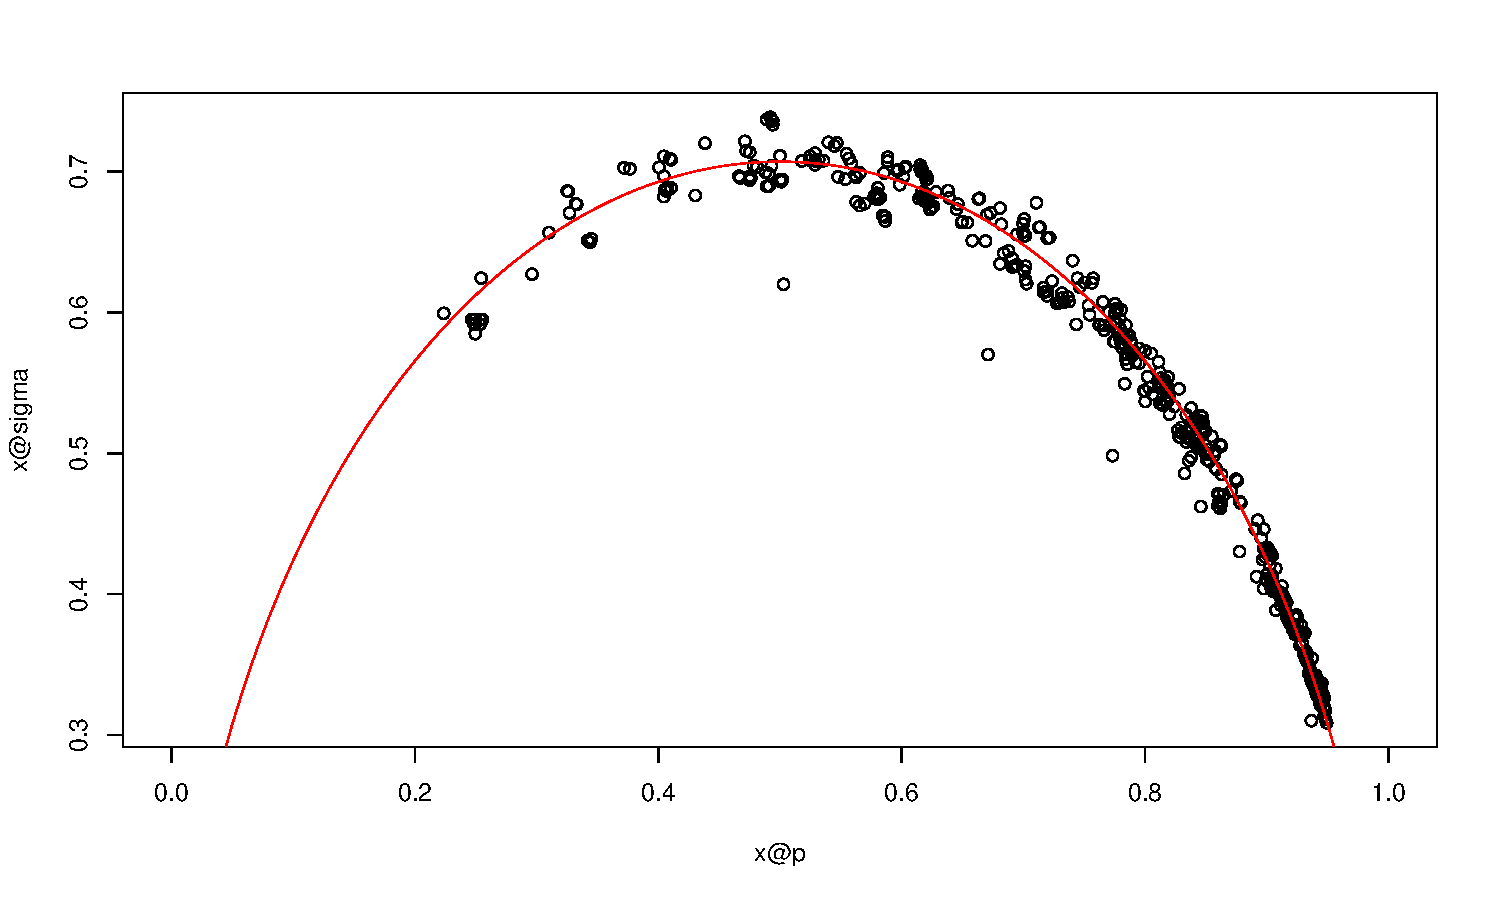
\includegraphics[width=0.7\textwidth]{figure/unnamed-chunk-14-1} 

}



\end{knitrout}
%\end{center}

  There are also function \verb!set.stats.snps! and \verb!set.stats.ped! which
  update only \verb!x@snps! and \verb!x@ped!.

  The option \verb!gaston.auto.set.stats! can be useful when extracting 
  individuals from bed.matrices (seen next section): if
  \verb!gaston.auto.set.stats = FALSE!, the slots \verb!@p!, \verb!@mu! and \verb!@sigma!
  are left unaltered; in contrast, the default behavior is to call \verb!set.stats! 
  which recomputes the values of these slots. 
  Note that when using \verb!set.stats! ``manually'', one can use options to alter its behavior, 
  allowing to update only some slots. The following code illustrates this (remember that here 
  \verb!gaston.auto.set.stats = FALSE!) :

\begin{knitrout}
\definecolor{shadecolor}{rgb}{0.969, 0.969, 0.969}\color{fgcolor}\begin{kframe}
\begin{alltt}
\hlstd{> }\hlkwd{head}\hlstd{(x}\hlopt{@}\hlkwc{p}\hlstd{)}
\end{alltt}
\begin{verbatim}
[1] 0.9025845 0.7664016 0.8399602 0.9433400 0.9433400 0.9423459
\end{verbatim}
\begin{alltt}
\hlstd{> }\hlstd{y} \hlkwb{<-} \hlstd{x[}\hlnum{1}\hlopt{:}\hlnum{30}\hlstd{,]}
\hlstd{> }\hlkwd{head}\hlstd{(y}\hlopt{@}\hlkwc{p}\hlstd{)}
\end{alltt}
\begin{verbatim}
[1] 0.9025845 0.7664016 0.8399602 0.9433400 0.9433400 0.9423459
\end{verbatim}
\begin{alltt}
\hlstd{> }\hlstd{y} \hlkwb{<-} \hlkwd{set.stats}\hlstd{(y,} \hlkwc{set.p} \hlstd{=} \hlnum{FALSE}\hlstd{)}
\end{alltt}
\begin{verbatim}
ped stats and snps stats have been set. 
'mu' and 'sigma' have been set.
\end{verbatim}
\begin{alltt}
\hlstd{> }\hlkwd{head}\hlstd{(y}\hlopt{@}\hlkwc{p}\hlstd{)}
\end{alltt}
\begin{verbatim}
[1] 0.9025845 0.7664016 0.8399602 0.9433400 0.9433400 0.9423459
\end{verbatim}
\begin{alltt}
\hlstd{> }\hlstd{y} \hlkwb{<-} \hlkwd{set.stats}\hlstd{(y)}
\end{alltt}
\begin{verbatim}
ped stats and snps stats have been set. 
'p' has been set. 
'mu' and 'sigma' have been set.
\end{verbatim}
\begin{alltt}
\hlstd{> }\hlkwd{head}\hlstd{(y}\hlopt{@}\hlkwc{p}\hlstd{)}
\end{alltt}
\begin{verbatim}
[1] 0.8833333 0.8000000 0.8166667 0.9833333 0.9833333 0.9833333
\end{verbatim}
\end{kframe}
\end{knitrout}

  Hardy-Weinberg Equilibrium can be tested for all SNPs simply by \verb!x <- set.hwe(x)!. 
  This command adds to the data frame \verb!x@snps! a column \verb!hwe!, containing the
  $p$-value of the test (both $\chi^2$ and ``exact'' tests are available, see the man
  page).

  Note that when writting a bed.matrix \verb!x! to disk with \verb!write.bed.matrix!, 
  the \verb!.rds! file contains all the slots of \verb!x!, and thus contains the additionnal
  variables added by \verb!set.stats! or \verb!set.hwe!, which are not saved in the
  \verb!.bim! and \verb!.fam! files.

  For the remaining of this vignette, we restore the default behaviour:
\begin{knitrout}
\definecolor{shadecolor}{rgb}{0.969, 0.969, 0.969}\color{fgcolor}\begin{kframe}
\begin{alltt}
\hlstd{> }\hlkwd{options}\hlstd{(}\hlkwc{gaston.auto.set.stats} \hlstd{=} \hlnum{TRUE}\hlstd{)}
\end{alltt}
\end{kframe}
\end{knitrout}

\pagebreak
\subsection{Subsetting bed.matrices}

  It is possible to subset bed.matrices just as normal matrices, writing e.g.
  \verb!x[1:100,]! to extract the first 100 individuals, or \verb!x[1:100,10:19]!
  to extract the SNPs 10 to 19 for these 100 individuals:

\begin{knitrout}
\definecolor{shadecolor}{rgb}{0.969, 0.969, 0.969}\color{fgcolor}\begin{kframe}
\begin{alltt}
\hlstd{> }\hlstd{x[}\hlnum{1}\hlopt{:}\hlnum{100}\hlstd{,]}
\end{alltt}
\begin{verbatim}
A bed.matrix with 100 individuals and 733 markers.
snps stats are set
ped stats are set
\end{verbatim}
\begin{alltt}
\hlstd{> }\hlstd{x[}\hlnum{1}\hlopt{:}\hlnum{100}\hlstd{,}\hlnum{10}\hlopt{:}\hlnum{19}\hlstd{]}
\end{alltt}
\begin{verbatim}
A bed.matrix with 100 individuals and 10 markers.
snps stats are set
ped stats are set
\end{verbatim}
\end{kframe}
\end{knitrout}

  The use of logical vectors for subsetting is allowed too. The following code extracts 
  the SNPs with minor allele frequency $> 0.1$:

\begin{knitrout}
\definecolor{shadecolor}{rgb}{0.969, 0.969, 0.969}\color{fgcolor}\begin{kframe}
\begin{alltt}
\hlstd{> }\hlstd{x[,x}\hlopt{@}\hlkwc{snps}\hlopt{$}\hlstd{maf} \hlopt{>} \hlnum{0.1}\hlstd{]}
\end{alltt}
\begin{verbatim}
A bed.matrix with 503 individuals and 501 markers.
snps stats are set
ped stats are set
\end{verbatim}
\end{kframe}
\end{knitrout}

  For this kind of selection, Gaston provides the functions \verb!select.inds! and 
  \verb!select.snps!, which have a nicer syntax. Hereafter 
  we use the same condition on the minor allele frequency, and we introduce also 
  a condition on the Hardy-Weinberg Equilibrium $p$-value:

\begin{knitrout}
\definecolor{shadecolor}{rgb}{0.969, 0.969, 0.969}\color{fgcolor}\begin{kframe}
\begin{alltt}
\hlstd{> }\hlstd{x} \hlkwb{<-} \hlkwd{set.hwe}\hlstd{(x)}
\end{alltt}
\begin{verbatim}
Computing HW chi-square p-values
\end{verbatim}
\begin{alltt}
\hlstd{> }\hlkwd{select.snps}\hlstd{(x, maf} \hlopt{>} \hlnum{0.1} \hlopt{&} \hlstd{hwe} \hlopt{>} \hlnum{1e-3}\hlstd{)}
\end{alltt}
\begin{verbatim}
A bed.matrix with 503 individuals and 497 markers.
snps stats are set
ped stats are set
\end{verbatim}
\end{kframe}
\end{knitrout}
  The conditions in \verb!select.snps! can use any of the variables defined in the data frame \verb!x@snps!,
  as well as variables defined in the user session. 

  The function \verb!select.inds! is similar, using variables of the data frame \verb!x@ped!. 
  One can for example 
  select individuals with callrate greater than 95\% with \verb!select.inds(x, callrate > 0.5)!.

  These functions should make basic Quality Control easy. 

  \noindent{\bfseries Note:}\ \ If \verb!options(gaston.auto.set.stats = FALSE)!
  was set, subsetting will erase some or all statistics added by \verb!set.stats!,
  except the \verb!p!, \verb!mu! and \verb!sigma! slots. 

\subsection{Genomic sex}
  When dealing with genome wide data,
  the function \verb!set.genomic.sex! can be use to add a \verb!x@ped$genomic.sex! column,
  determined by clustering on individuals X heterozygosity rate and Y callrate.
 
  \verb!x <- select.inds(x, sex == genomic.sex)! will then allow to keep only individuals 
  whose sex and genomic sex are concordant.

  An other possibility is to use \verb!x@ped$sex <- x@ped$genomic.sex; x <- set.stats(x)! 
  to erase the original sex indication and use genomic sex in subsequent analyses.

\subsection{Merging bed.matrices}

  Gaston defines methods \verb!rbind! and \verb!cbind! which can be used to merge several
  bed.matrices. \verb!cbind! checks that individuals famids and ids are identical ; all remaining
  columns are taken from the first argument, without further control.

\begin{knitrout}
\definecolor{shadecolor}{rgb}{0.969, 0.969, 0.969}\color{fgcolor}\begin{kframe}
\begin{alltt}
\hlstd{> }\hlkwd{data}\hlstd{(AGT)}
\hlstd{> }\hlstd{x1} \hlkwb{<-} \hlkwd{as.bed.matrix}\hlstd{(AGT.gen, AGT.fam, AGT.bim)}
\hlstd{> }\hlstd{x1}
\end{alltt}
\begin{verbatim}
A bed.matrix with 503 individuals and 361 markers.
snps stats are set
ped stats are set
\end{verbatim}
\begin{alltt}
\hlstd{> }\hlkwd{data}\hlstd{(LCT)}
\hlstd{> }\hlstd{x2} \hlkwb{<-} \hlkwd{as.bed.matrix}\hlstd{(LCT.gen, LCT.fam, LCT.bim)}
\hlstd{> }\hlstd{x2}
\end{alltt}
\begin{verbatim}
A bed.matrix with 503 individuals and 607 markers.
snps stats are set
ped stats are set
\end{verbatim}
\begin{alltt}
\hlstd{> }\hlstd{x} \hlkwb{<-} \hlkwd{cbind}\hlstd{(x1,x2)}
\hlstd{> }\hlstd{x}
\end{alltt}
\begin{verbatim}
A bed.matrix with 503 individuals and 968 markers.
snps stats are set
ped stats are set
\end{verbatim}
\end{kframe}
\end{knitrout}

  \verb!rbind! similarly checks whether the SNP ids are identical, and also if the reference
  alleles are identical. If needed, it will perform reference allele inversions (changing a SNP
  A/G to G/A) or allele strand flips (changing A/G to T/C) or both.

\begin{knitrout}
\definecolor{shadecolor}{rgb}{0.969, 0.969, 0.969}\color{fgcolor}\begin{kframe}
\begin{alltt}
\hlstd{> }\hlstd{x3} \hlkwb{<-} \hlstd{x[}\hlnum{1}\hlopt{:}\hlnum{10}\hlstd{, ]}
\hlstd{> }\hlstd{x4} \hlkwb{<-} \hlstd{x[}\hlopt{-}\hlstd{(}\hlnum{1}\hlopt{:}\hlnum{10}\hlstd{), ]}
\hlstd{> }\hlkwd{rbind}\hlstd{(x3,x4)}
\end{alltt}
\begin{verbatim}
A bed.matrix with 503 individuals and 968 markers.
snps stats are set
ped stats are set
\end{verbatim}
\end{kframe}
\end{knitrout}


%%%%%%%%%%%%%%%%%%%%%%%%%%%%%%%%%%%%%%%%%%%%%%%%%%%%%%%%%%%%%%%%%%%%%%%%%%%%%%%%%%%%%%%%%%%%%%%%%%%%
\section{Standardized matrices}

  Gaston allows to ``standardize'' a genotype matrix, replacing each genotype $X_{ij}$ ($i$ is the
  individual index, $j$ is the SNP index) by 
\begin{equation}
X_{ij} - \mu_j \over \sigma_j
\end{equation}
  where $\mu_j = 2 p_j$ is the mean of the 0,1,2-coded genotype ($p_j$ being the alternate allele 
  frequency), and $\sigma_j$ is either its standard error, or the expected standard error under Hardy-Weinberg
  Equilibrium, that is $\sqrt{2p_j(1-p_j)}$.

  Consider the TTN data set. The unscaled matrix contains 0,1,2 values:
\begin{knitrout}
\definecolor{shadecolor}{rgb}{0.969, 0.969, 0.969}\color{fgcolor}\begin{kframe}
\begin{alltt}
\hlstd{> }\hlstd{x} \hlkwb{<-} \hlkwd{as.bed.matrix}\hlstd{(TTN.gen, TTN.fam, TTN.bim)}
\hlstd{> }\hlstd{X} \hlkwb{<-} \hlkwd{as.matrix}\hlstd{(x)}
\hlstd{> }\hlstd{X[}\hlnum{1}\hlopt{:}\hlnum{5}\hlstd{,}\hlnum{1}\hlopt{:}\hlnum{4}\hlstd{]}
\end{alltt}
\begin{verbatim}
        rs7571247 rs3813253 rs6760059 rs16866263
HG00096         2         2         2          2
HG00097         2         2         2          2
HG00099         1         2         2          2
HG00100         2         0         0          2
HG00101         2         2         2          2
\end{verbatim}
\end{kframe}
\end{knitrout}

  To scale it using the standard error, use \verb!standardize(x) <- "mu_sigma"! (or \verb!standardize(x) <- "mu"!,
  as the function uses \verb!match.arg!):
\begin{knitrout}
\definecolor{shadecolor}{rgb}{0.969, 0.969, 0.969}\color{fgcolor}\begin{kframe}
\begin{alltt}
\hlstd{> }\hlkwd{standardize}\hlstd{(x)} \hlkwb{<-} \hlstr{"mu"}
\hlstd{> }\hlkwd{as.matrix}\hlstd{(x)[}\hlnum{1}\hlopt{:}\hlnum{5}\hlstd{,} \hlnum{1}\hlopt{:}\hlnum{4}\hlstd{]}
\end{alltt}
\begin{verbatim}
         rs7571247  rs3813253  rs6760059 rs16866263
HG00096  0.4629595  0.7953656  0.6254622  0.3437939
HG00097  0.4629595  0.7953656  0.6254622  0.3437939
HG00099 -1.9132512  0.7953656  0.6254622  0.3437939
HG00100  0.4629595 -2.6094762 -3.2827052  0.3437939
HG00101  0.4629595  0.7953656  0.6254622  0.3437939
\end{verbatim}
\end{kframe}
\end{knitrout}

  The result is similar to what would be obtained from the base function \verb!scale!:
\begin{knitrout}
\definecolor{shadecolor}{rgb}{0.969, 0.969, 0.969}\color{fgcolor}\begin{kframe}
\begin{alltt}
\hlstd{> }\hlkwd{scale}\hlstd{(X)[}\hlnum{1}\hlopt{:}\hlnum{5}\hlstd{,}\hlnum{1}\hlopt{:}\hlnum{4}\hlstd{]}
\end{alltt}
\begin{verbatim}
         rs7571247  rs3813253  rs6760059 rs16866263
HG00096  0.4629595  0.7953656  0.6254622  0.3437939
HG00097  0.4629595  0.7953656  0.6254622  0.3437939
HG00099 -1.9132512  0.7953656  0.6254622  0.3437939
HG00100  0.4629595 -2.6094762 -3.2827052  0.3437939
HG00101  0.4629595  0.7953656  0.6254622  0.3437939
\end{verbatim}
\end{kframe}
\end{knitrout}

  To use $\sqrt{2p_j(1-p_j)}$ instead of the standard error, use \verb!standardize(x) <- "p"!; a similar
  result can again be obtained from \verb!scale!, with the right options:
\begin{knitrout}
\definecolor{shadecolor}{rgb}{0.969, 0.969, 0.969}\color{fgcolor}\begin{kframe}
\begin{alltt}
\hlstd{> }\hlkwd{standardize}\hlstd{(x)} \hlkwb{<-} \hlstr{"p"}
\hlstd{> }\hlkwd{as.matrix}\hlstd{(x)[}\hlnum{1}\hlopt{:}\hlnum{5}\hlstd{,} \hlnum{1}\hlopt{:}\hlnum{4}\hlstd{]}
\end{alltt}
\begin{verbatim}
         rs7571247  rs3813253  rs6760059 rs16866263
HG00096  0.4646063  0.7807675  0.6173047  0.3465926
HG00097  0.4646063  0.7807675  0.6173047  0.3465926
HG00099 -1.9200567  0.7807675  0.6173047  0.3465926
HG00100  0.4646063 -2.5615820 -3.2398911  0.3465926
HG00101  0.4646063  0.7807675  0.6173047  0.3465926
\end{verbatim}
\begin{alltt}
\hlstd{> }\hlkwd{scale}\hlstd{(X,} \hlkwc{scale} \hlstd{=} \hlkwd{sqrt}\hlstd{(}\hlnum{2}\hlopt{*}\hlstd{x}\hlopt{@}\hlkwc{p}\hlopt{*}\hlstd{(}\hlnum{1}\hlopt{-}\hlstd{x}\hlopt{@}\hlkwc{p}\hlstd{)))[}\hlnum{1}\hlopt{:}\hlnum{5}\hlstd{,}\hlnum{1}\hlopt{:}\hlnum{4}\hlstd{]}
\end{alltt}
\begin{verbatim}
         rs7571247  rs3813253  rs6760059 rs16866263
HG00096  0.4646063  0.7807675  0.6173047  0.3465926
HG00097  0.4646063  0.7807675  0.6173047  0.3465926
HG00099 -1.9200567  0.7807675  0.6173047  0.3465926
HG00100  0.4646063 -2.5615820 -3.2398911  0.3465926
HG00101  0.4646063  0.7807675  0.6173047  0.3465926
\end{verbatim}
\end{kframe}
\end{knitrout}

  To go back to the 0,1,2-coded genotypes, use \verb!standardize(x) <- "none"!.

  \noindent{\bfseries Note:}\ \ In standardized matrices, the \verb!NA! values are replaced by zeroes,
  which amount to impute the missing genotypes by the mean genotype.

\subsection{Matrix multiplication}

  Standardized matrices can be multiplied with numeric vectors or matrices with the operator \verb!%*%!.

  This feature can be used e.g. to simulate quantitative phenotypes with a genetic component. The following
  code simulates a phenotype with an effect of the SNP \#350:
\begin{knitrout}
\definecolor{shadecolor}{rgb}{0.969, 0.969, 0.969}\color{fgcolor}\begin{kframe}
\begin{alltt}
\hlstd{> }\hlstd{y} \hlkwb{<-} \hlstd{x} \hlopt \hlkwd{c}\hlstd{(}\hlkwd{rep}\hlstd{(}\hlnum{0}\hlstd{,}\hlnum{350}\hlstd{),}\hlnum{0.25}\hlstd{,}\hlkwd{rep}\hlstd{(}\hlnum{0}\hlstd{,}\hlkwd{ncol}\hlstd{(x)}\hlopt{-}\hlnum{351}\hlstd{))} \hlopt{+} \hlkwd{rnorm}\hlstd{(}\hlkwd{nrow}\hlstd{(x),} \hlkwc{sd} \hlstd{=} \hlnum{1}\hlstd{)}
\end{alltt}
\end{kframe}
\end{knitrout}

\pagebreak
\subsection{Genetic Relationship Matrix and Principal Component Analysis}

  If $X_s$ is a standardized $n\times q$ genotype matrix, a Genetic Relationship Matrix 
  (GRM) of the individuals can be computed as
  \begin{equation*}
     GRM = {1\over q-1} X_sX_s'
  \end{equation*}
  where $q$ is the number of SNPs.  This computation is done by the function \verb!GRM!.  

  \textbf{NOTE:} Since version 1.4.7, \verb!GRM! has an argument \verb!which.snps! which allows 
  to give a logical vector specifying which SNPs to use in the computation. The default is to 
  use only autosomal SNPs (the above formula makes little to no sense for X linked SNPs, unless there 
  are only women in the sample).

  The Principal Component Analysis (PCA) of large genomic data sets is used to retrieve population
  stratification. It can be obtained from the eigen decomposition of the GRM. To illustrate this,
  we included in the \verb!extdata! folder a dataset extracted from the 1000 genomes project. 
  This data set comprehend the 503 individuals of european ascent, with 10025 SNPs on the chromosome
  2. These SNPs have been selected with the function \verb!LD.thin! so that they have very low 
  LD with each other ($r^2 < 0.05$). We added in the data frame \verb!x@ped! a variable \verb!population!
  which is a factor with levels \verb!CEU!, \verb!FIN!, \verb!GBR!, \verb!IBS! and \verb!TSI!.

  We can load this data set as follows:
\begin{knitrout}
\definecolor{shadecolor}{rgb}{0.969, 0.969, 0.969}\color{fgcolor}\begin{kframe}
\begin{alltt}
\hlstd{> }\hlstd{x} \hlkwb{<-} \hlkwd{read.bed.matrix}\hlstd{(} \hlkwd{system.file}\hlstd{(}\hlstr{"extdata"}\hlstd{,} \hlstr{"chr2.bed"}\hlstd{,} \hlkwc{package}\hlstd{=}\hlstr{"gaston"}\hlstd{) )}
\end{alltt}
\begin{verbatim}
Reading /home/rv/R/R-3.4/gaston/extdata/chr2.rds 
Reading /home/rv/R/R-3.4/gaston/extdata/chr2.bed 
\end{verbatim}
\begin{alltt}
\hlstd{> }\hlstd{x}
\end{alltt}
\begin{verbatim}
A bed.matrix with 503 individuals and 10025 markers.
snps stats are not set (or incomplete)
ped stats are not set (or incomplete)
\end{verbatim}
\begin{alltt}
\hlstd{> }\hlkwd{head}\hlstd{(x}\hlopt{@}\hlkwc{ped}\hlstd{)}
\end{alltt}
\begin{verbatim}
    famid      id father mother sex pheno population
1 HG00096 HG00096      0      0   0    -9        GBR
2 HG00097 HG00097      0      0   0    -9        GBR
3 HG00099 HG00099      0      0   0    -9        GBR
4 HG00100 HG00100      0      0   0    -9        GBR
5 HG00101 HG00101      0      0   0    -9        GBR
6 HG00102 HG00102      0      0   0    -9        GBR
\end{verbatim}
\begin{alltt}
\hlstd{> }\hlkwd{table}\hlstd{(x}\hlopt{@}\hlkwc{ped}\hlopt{$}\hlstd{population)}
\end{alltt}
\begin{verbatim}

CEU FIN GBR IBS TSI 
 99  99  91 107 107 
\end{verbatim}
\end{kframe}
\end{knitrout}


We compute the Genetic Relationship Matrix, and its eigen decomposition (we don't
need to standardize \verb!x! explicitely: is \verb!x! isn't standardized, 
\verb!GRM! will use \verb!standardize(x) = "p"!):
\begin{knitrout}
\definecolor{shadecolor}{rgb}{0.969, 0.969, 0.969}\color{fgcolor}\begin{kframe}
\begin{alltt}
\hlstd{> }\hlstd{K} \hlkwb{<-} \hlkwd{GRM}\hlstd{(x)}
\hlstd{> }
\hlstd{> }\hlstd{eiK} \hlkwb{<-} \hlkwd{eigen}\hlstd{(K)}
\hlstd{> }\hlcom{# deal with a small negative eigen value}
\hlstd{> }\hlstd{eiK}\hlopt{$}\hlstd{values[ eiK}\hlopt{$}\hlstd{values} \hlopt{<} \hlnum{0} \hlstd{]} \hlkwb{<-} \hlnum{0}
\end{alltt}
\end{kframe}
\end{knitrout}

  The eigenvectors are normalized. The Principal Components (PC) can be computed by 
  multiplying them by the square root of the associated eigenvalues. Here we plot
  the projection of the 503 individuals on the first two PCs, with colors corresponding
  to their population.

%\begin{center}
\begin{knitrout}
\definecolor{shadecolor}{rgb}{0.969, 0.969, 0.969}\color{fgcolor}\begin{kframe}
\begin{alltt}
\hlstd{> }\hlstd{PC} \hlkwb{<-} \hlkwd{sweep}\hlstd{(eiK}\hlopt{$}\hlstd{vectors,} \hlnum{2}\hlstd{,} \hlkwd{sqrt}\hlstd{(eiK}\hlopt{$}\hlstd{values),} \hlstr{"*"}\hlstd{)}
\hlstd{> }\hlkwd{plot}\hlstd{(PC[,}\hlnum{1}\hlstd{], PC[,}\hlnum{2}\hlstd{],} \hlkwc{col}\hlstd{=x}\hlopt{@}\hlkwc{ped}\hlopt{$}\hlstd{population)}
\hlstd{> }\hlkwd{legend}\hlstd{(}\hlstr{"bottomleft"}\hlstd{,} \hlkwc{pch} \hlstd{=} \hlnum{1}\hlstd{,} \hlkwc{legend} \hlstd{=} \hlkwd{levels}\hlstd{(x}\hlopt{@}\hlkwc{ped}\hlopt{$}\hlstd{population),} \hlkwc{col} \hlstd{=} \hlnum{1}\hlopt{:}\hlnum{5}\hlstd{)}
\end{alltt}
\end{kframe}

{\centering 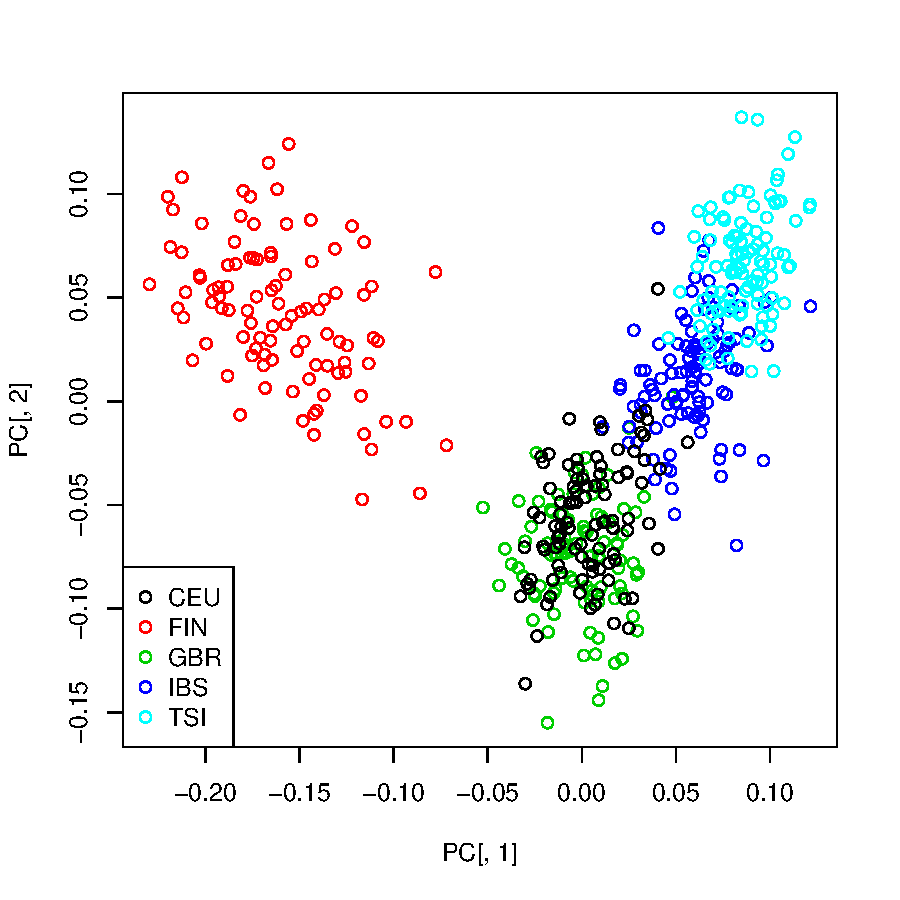
\includegraphics[width=0.4\textwidth]{figure/unnamed-chunk-29-1} 

}



\end{knitrout}
%\end{center}

  As $K$ can be written
  \begin{equation*} 
    K = \left( {1 \over \sqrt{q-1}} X_s \right) \left( {1 \over \sqrt{q-1}} X_s \right)',
  \end{equation*}
  the PCs are the left singular vectors of ${1 \over \sqrt{q-1}} X_s$.
  The vectors of loadings are the right singlar vectors of this matrix. The vector of loadings 
  corresponding to a PC $u$ is the vector $v$ with unit norm, such that 
  $u = {1 \over \sqrt{q-1}} X_s v$.

  They can be retrieved with the function \verb!bed.loadings!:
\begin{knitrout}
\definecolor{shadecolor}{rgb}{0.969, 0.969, 0.969}\color{fgcolor}\begin{kframe}
\begin{alltt}
\hlstd{> }\hlcom{# one can use PC[,1:2] instead of eiK$vectors[,1:2] as well}
\hlstd{> }\hlstd{L} \hlkwb{<-} \hlkwd{bed.loadings}\hlstd{(x, eiK}\hlopt{$}\hlstd{vectors[,}\hlnum{1}\hlopt{:}\hlnum{2}\hlstd{])}
\hlstd{> }\hlkwd{dim}\hlstd{(L)}
\end{alltt}
\begin{verbatim}
[1] 10025     2
\end{verbatim}
\begin{alltt}
\hlstd{> }\hlkwd{head}\hlstd{(L)}
\end{alltt}
\begin{verbatim}
                     [,1]          [,2]
rs113106463  0.0059549201  0.0064476344
rs13390778   0.0099678236 -0.0125721014
rs75011129   0.0001122793 -0.0001181844
rs4637157    0.0151318053 -0.0148076772
rs62116661   0.0002977573  0.0048268309
rs10170011  -0.0185198431 -0.0019553418
\end{verbatim}
\end{kframe}
\end{knitrout}

We verify that the loadings have unit norm:
\begin{knitrout}
\definecolor{shadecolor}{rgb}{0.969, 0.969, 0.969}\color{fgcolor}\begin{kframe}
\begin{alltt}
\hlstd{> }\hlkwd{colSums}\hlstd{(L}\hlopt{**}\hlnum{2}\hlstd{)}
\end{alltt}
\begin{verbatim}
[1] 1 1
\end{verbatim}
\end{kframe}
\end{knitrout}

And that the PCs are retrieved by right multiplying $X_s$ by the loadings (here we need 
to explicitely standardize \verb!x!):
\begin{knitrout}
\definecolor{shadecolor}{rgb}{0.969, 0.969, 0.969}\color{fgcolor}\begin{kframe}
\begin{alltt}
\hlstd{> }\hlkwd{standardize}\hlstd{(x)} \hlkwb{<-} \hlstr{'p'}
\hlstd{> }\hlkwd{head}\hlstd{( (x} \hlopt \hlstd{L)} \hlopt{/} \hlkwd{sqrt}\hlstd{(}\hlkwd{ncol}\hlstd{(x)}\hlopt{-}\hlnum{1}\hlstd{) )}
\end{alltt}
\begin{verbatim}
                [,1]        [,2]
HG00096 -0.021410863 -0.12418398
HG00097  0.014005030 -0.07378042
HG00099 -0.001384432 -0.09708208
HG00100 -0.020319164 -0.08920828
HG00101 -0.002596083 -0.08925961
HG00102 -0.010155031 -0.08968427
\end{verbatim}
\begin{alltt}
\hlstd{> }\hlkwd{head}\hlstd{( PC[,}\hlnum{1}\hlopt{:}\hlnum{2}\hlstd{] )}
\end{alltt}
\begin{verbatim}
             [,1]        [,2]
[1,] -0.021410843 -0.12418392
[2,]  0.014005028 -0.07378041
[3,] -0.001384429 -0.09708204
[4,] -0.020319171 -0.08920827
[5,] -0.002596078 -0.08925959
[6,] -0.010155008 -0.08968426
\end{verbatim}
\end{kframe}
\end{knitrout}


\vfill\eject
\subsection{Linkage Disequilibrium}

  Doing the crossproduct in the reverse order produces a moment estimate of the 
  Linkage Disequilibrium (LD):
  \begin{equation*} 
    LD = {1\over n-1} X_s'X_s 
  \end{equation*}
  where $n$ is the number of individuals. This computation is done by the function
  \verb!LD! (usually, only parts of the whole LD matrix is computed).  
  The fonction \verb!LD! can compute a square symmetric matrix giving the LD for a given 
  region, measured by $r^2$ (the default), $r$ or $D$. It can also compute the LD  between
  two different regions.

\begin{center}
\setkeys{Gin}{width=\textwidth}
\begin{knitrout}
\definecolor{shadecolor}{rgb}{0.969, 0.969, 0.969}\color{fgcolor}\begin{kframe}
\begin{alltt}
\hlstd{> }\hlkwd{data}\hlstd{(AGT)}
\hlstd{> }\hlstd{x} \hlkwb{<-} \hlkwd{as.bed.matrix}\hlstd{(AGT.gen, AGT.fam, AGT.bim)}
\hlstd{> }
\hlstd{> }\hlstd{ld.x} \hlkwb{<-} \hlkwd{LD}\hlstd{(x,} \hlkwd{c}\hlstd{(}\hlnum{1}\hlstd{,}\hlkwd{ncol}\hlstd{(x)))}
\hlstd{> }
\hlstd{> }\hlkwd{LD.plot}\hlstd{(ld.x,} \hlkwc{snp.positions} \hlstd{= x}\hlopt{@}\hlkwc{snps}\hlopt{$}\hlstd{pos,} \hlkwc{write.ld} \hlstd{=} \hlkwa{NULL}\hlstd{,}
\hlstd{+ }        \hlkwc{max.dist} \hlstd{=} \hlnum{20e3}\hlstd{,} \hlkwc{write.snp.id} \hlstd{=} \hlnum{FALSE}\hlstd{,} \hlkwc{draw.chr} \hlstd{=} \hlnum{FALSE}\hlstd{,}
\hlstd{+ }        \hlkwc{pdf} \hlstd{=} \hlstr{"LD_AGT.pdf"}\hlstd{)}
\end{alltt}
\begin{verbatim}
pdf 
  2 
\end{verbatim}
\end{kframe}
\end{knitrout}
\includegraphics[width=\textwidth]{LD_AGT.pdf}
\end{center}

  This method is 
  also used by \verb!LD.thin! to extract a set of SNPs in low linkage disequilibrium
  (it is often recommended to perform this operation before computing the GRM). We illustrate
  this function on the AGT data set:

\begin{knitrout}
\definecolor{shadecolor}{rgb}{0.969, 0.969, 0.969}\color{fgcolor}\begin{kframe}
\begin{alltt}
\hlstd{> }\hlstd{y} \hlkwb{<-} \hlkwd{LD.thin}\hlstd{(x,} \hlkwc{threshold} \hlstd{=} \hlnum{0.4}\hlstd{,} \hlkwc{max.dist} \hlstd{=} \hlnum{500e3}\hlstd{)}
\hlstd{> }\hlstd{y}
\end{alltt}
\begin{verbatim}
A bed.matrix with 503 individuals and 48 markers.
snps stats are set
ped stats are set
\end{verbatim}
\end{kframe}
\end{knitrout}

The argument \verb!max.dist = 500e3! is to specify that the LD won't be computed for
SNPs more than 500 kb appart. We verify that there is no SNP pair with LD $r^2 > 0.4$
(note that the LD matrix has ones on the diagonal):

\begin{knitrout}
\definecolor{shadecolor}{rgb}{0.969, 0.969, 0.969}\color{fgcolor}\begin{kframe}
\begin{alltt}
\hlstd{> }\hlstd{ld.y} \hlkwb{<-} \hlkwd{LD}\hlstd{( y,} \hlkwc{lim} \hlstd{=} \hlkwd{c}\hlstd{(}\hlnum{1}\hlstd{,} \hlkwd{ncol}\hlstd{(y)) )}
\hlstd{> }\hlkwd{sum}\hlstd{( ld.y} \hlopt{>} \hlnum{0.4} \hlstd{)}
\end{alltt}
\begin{verbatim}
[1] 48
\end{verbatim}
\end{kframe}
\end{knitrout}

%%%%%%%%%%%%%%%%%%%%%%%%%%%%%%%%%%%%%%%%%%%%%%%%%%%%%%%%%%%%%%%%%%%%%%%%%%%%%%%%%%%%%%%%%%%%%%%%%%%%
\vfill\eject
\section{Linear Mixed Models}

\def\R{\mathbb{R}}
\def\N{\mathcal{N}}

  Linear Mixed Models are usually written under the form
  \begin{equation*}
    Y = X\beta + Z_1 u_1 + \cdots + Z_k u_k + \varepsilon
  \end{equation*}
  where $Y \in\R^{n}$ is the response vector, and $X\in \R^{n\times p}, Z_1 \in \R^{n\times q_1}, \dots, Z_k \in\R^{n\times q_k}$ are
  design matrices. The vector $\beta\in\R^p$ is the vector of fixed effects; the random effects are drawn in 
  normal distributions, $u_1\sim \N(0, \tau_1 I_{q_1}), \dots, u_k\sim \N(0, \tau_k I_{q_k})$, as the residual
  error $\epsilon\sim\N(0,\sigma^2 I_n)$.

  Here we will use the equivalent form 
  \begin{equation*}
    Y = X\beta + \omega_1 + \ldots + \omega_k + \varepsilon
  \end{equation*}
  where $K_i = Z_i Z_i'$ $(i = 1, \dots, k)$,
  the random terms are $\omega_i \sim N(0,\tau_i K_i)$ for $i \in 1, \dots,k$ and $\varepsilon \sim N(0,\sigma^2 I_n)$.

  Note that using the R function \verb!model.matrix! can help you to rewrite a model under this form.

  Gaston provides two functions for estimating the model parameters when the model is
  written in the second form. We are going to illustrate these functions on simulated
  data.

  \subsection{Data simulation}

  We will use the above notations. First generate some (random) design matrices:
 
\begin{knitrout}
\definecolor{shadecolor}{rgb}{0.969, 0.969, 0.969}\color{fgcolor}\begin{kframe}
\begin{alltt}
\hlstd{> }\hlkwd{set.seed}\hlstd{(}\hlnum{1}\hlstd{)}
\hlstd{> }\hlstd{n} \hlkwb{<-} \hlnum{100}
\hlstd{> }\hlstd{q1} \hlkwb{<-} \hlnum{20}
\hlstd{> }\hlstd{Z1} \hlkwb{<-} \hlkwd{matrix}\hlstd{(} \hlkwd{rnorm}\hlstd{(n}\hlopt{*}\hlstd{q1),} \hlkwc{nrow} \hlstd{= n )}
\hlstd{> }\hlstd{X} \hlkwb{<-} \hlkwd{cbind}\hlstd{(}\hlnum{1}\hlstd{,} \hlnum{5}\hlopt{*}\hlkwd{runif}\hlstd{(n))}
\end{alltt}
\end{kframe}
\end{knitrout}
 
  Then the vector of random effects $u_1$ and a vector $y$ under the model $Y = X (1,2)' + Z u_1 + \varepsilon$
  with $u_1 \sim \N(0, 2 I_{q_1})$ and $\varepsilon \sim\N(0, 3 I_n)$:

\begin{knitrout}
\definecolor{shadecolor}{rgb}{0.969, 0.969, 0.969}\color{fgcolor}\begin{kframe}
\begin{alltt}
\hlstd{> }\hlstd{u1} \hlkwb{<-} \hlkwd{rnorm}\hlstd{(q1,} \hlkwc{sd} \hlstd{=} \hlkwd{sqrt}\hlstd{(}\hlnum{2}\hlstd{))}
\hlstd{> }\hlstd{y} \hlkwb{<-} \hlstd{X} \hlopt \hlkwd{c}\hlstd{(}\hlnum{1}\hlstd{,}\hlnum{2}\hlstd{)} \hlopt{+} \hlstd{Z1} \hlopt \hlstd{u1} \hlopt{+} \hlkwd{rnorm}\hlstd{(n,} \hlkwc{sd} \hlstd{=} \hlkwd{sqrt}\hlstd{(}\hlnum{3}\hlstd{))}
\end{alltt}
\end{kframe}
\end{knitrout}

  To illustrate the case where there are several random effects vectors, we generate an 
  other matrix $Z_2$, the corresponding vector of random effects $u_2$, and a vector $y_2$ 
  under the model $Y = X (1,2)' + Z u_1 + Z_2 u_2 + \varepsilon$.

\begin{knitrout}
\definecolor{shadecolor}{rgb}{0.969, 0.969, 0.969}\color{fgcolor}\begin{kframe}
\begin{alltt}
\hlstd{> }\hlstd{q2} \hlkwb{<-} \hlnum{10}
\hlstd{> }\hlstd{Z2} \hlkwb{<-} \hlkwd{matrix}\hlstd{(} \hlkwd{rnorm}\hlstd{(n}\hlopt{*}\hlstd{q2),} \hlkwc{nrow} \hlstd{= n )}
\hlstd{> }\hlstd{u2} \hlkwb{<-} \hlkwd{rnorm}\hlstd{(q2,} \hlkwc{sd} \hlstd{=} \hlnum{1}\hlstd{)}
\hlstd{> }\hlstd{y2} \hlkwb{<-} \hlstd{X} \hlopt \hlkwd{c}\hlstd{(}\hlnum{1}\hlstd{,}\hlnum{2}\hlstd{)} \hlopt{+} \hlstd{Z1} \hlopt \hlstd{u1} \hlopt{+} \hlstd{Z2} \hlopt \hlstd{u2} \hlopt{+} \hlkwd{rnorm}\hlstd{(n,} \hlkwc{sd} \hlstd{=} \hlkwd{sqrt}\hlstd{(}\hlnum{3}\hlstd{))}
\end{alltt}
\end{kframe}
\end{knitrout}

  \subsection{Model fitting with the AIREML algorithm}

  \verb!lmm.aireml! is a function for linear mixed models parameter estimation
  and BLUP computations. 

  \subsubsection{One random effects vector}
  Let's start with the simple case (only one random effects vector).
  As  \verb!lmm.aireml! uses the second form of the linear mixed model,
  and we give it the matrix $K_1 = Z_1 Z_1'$.

\begin{knitrout}
\definecolor{shadecolor}{rgb}{0.969, 0.969, 0.969}\color{fgcolor}\begin{kframe}
\begin{alltt}
\hlstd{> }\hlstd{K1} \hlkwb{<-} \hlkwd{tcrossprod}\hlstd{(Z1)}
\hlstd{> }\hlstd{fit} \hlkwb{<-} \hlkwd{lmm.aireml}\hlstd{(y, X,} \hlkwc{K} \hlstd{= K1,} \hlkwc{verbose} \hlstd{=} \hlnum{FALSE}\hlstd{)}
\hlstd{> }\hlkwd{str}\hlstd{(fit)}
\end{alltt}
\begin{verbatim}
List of 11
 $ sigma2    : num 3.37
 $ tau       : num 1.65
 $ logL      : num -150
 $ logL0     : num -231
 $ niter     : int 8
 $ norm_grad : num 2.21e-08
 $ Py        : num [1:100] 0.509 -0.236 0.11 0.328 -0.291 ...
 $ BLUP_omega: num [1:100] -0.441 -12.618 -1.724 5.052 5.831 ...
 $ BLUP_beta : num [1:2] 1.4 1.79
 $ varbeta   : num [1:2, 1:2] 0.1398 -0.0403 -0.0403 0.0167
 $ varXbeta  : num 7.61
\end{verbatim}
\end{kframe}
\end{knitrout}

  The result is a list giving all kind of information. Here we see that $\tau$ is 
  estimated to $1.65$ and $\sigma^2$ to $3.37$. 
  The Best Linear Unbiased Predictor (BLUP) for $\beta$ is in the component \verb!BLUP_beta!
  and here it is $(1.4, 1.79)$.
  
  The component \verb!BLUP_omega! holds the BLUP for $\omega_1 = Z u_1$. The BLUP for $u_1$
  can be retrieved by the formula $\widehat{u_1} = \tau_1 Z_1' P y$, the value of $Py$ being
  in the component \verb!BLUP_Py!. The plots below compare the true values of $\omega_1$ and
  $u_1$ with their BLUPs.
   
%\setkeys{Gin}{width=0.7\textwidth}
%\begin{center}
\begin{knitrout}
\definecolor{shadecolor}{rgb}{0.969, 0.969, 0.969}\color{fgcolor}\begin{kframe}
\begin{alltt}
\hlstd{> }\hlkwd{par}\hlstd{(}\hlkwc{mfrow} \hlstd{=} \hlkwd{c}\hlstd{(}\hlnum{1}\hlstd{,} \hlnum{2}\hlstd{))}
\hlstd{> }\hlkwd{plot}\hlstd{(Z1} \hlopt \hlstd{u1, fit}\hlopt{$}\hlstd{BLUP_omega);} \hlkwd{abline}\hlstd{(}\hlnum{0}\hlstd{,} \hlnum{1}\hlstd{,} \hlkwc{lty} \hlstd{=} \hlnum{2}\hlstd{,} \hlkwc{col} \hlstd{=} \hlnum{3}\hlstd{)}
\hlstd{> }\hlstd{BLUP_u1} \hlkwb{<-} \hlstd{fit}\hlopt{$}\hlstd{tau} \hlopt{*} \hlkwd{t}\hlstd{(Z1)} \hlopt \hlstd{fit}\hlopt{$}\hlstd{Py}
\hlstd{> }\hlkwd{plot}\hlstd{(u1, BLUP_u1);} \hlkwd{abline}\hlstd{(}\hlnum{0}\hlstd{,} \hlnum{1}\hlstd{,} \hlkwc{lty} \hlstd{=} \hlnum{2}\hlstd{,} \hlkwc{col} \hlstd{=} \hlnum{3}\hlstd{)}
\end{alltt}
\end{kframe}

{\centering 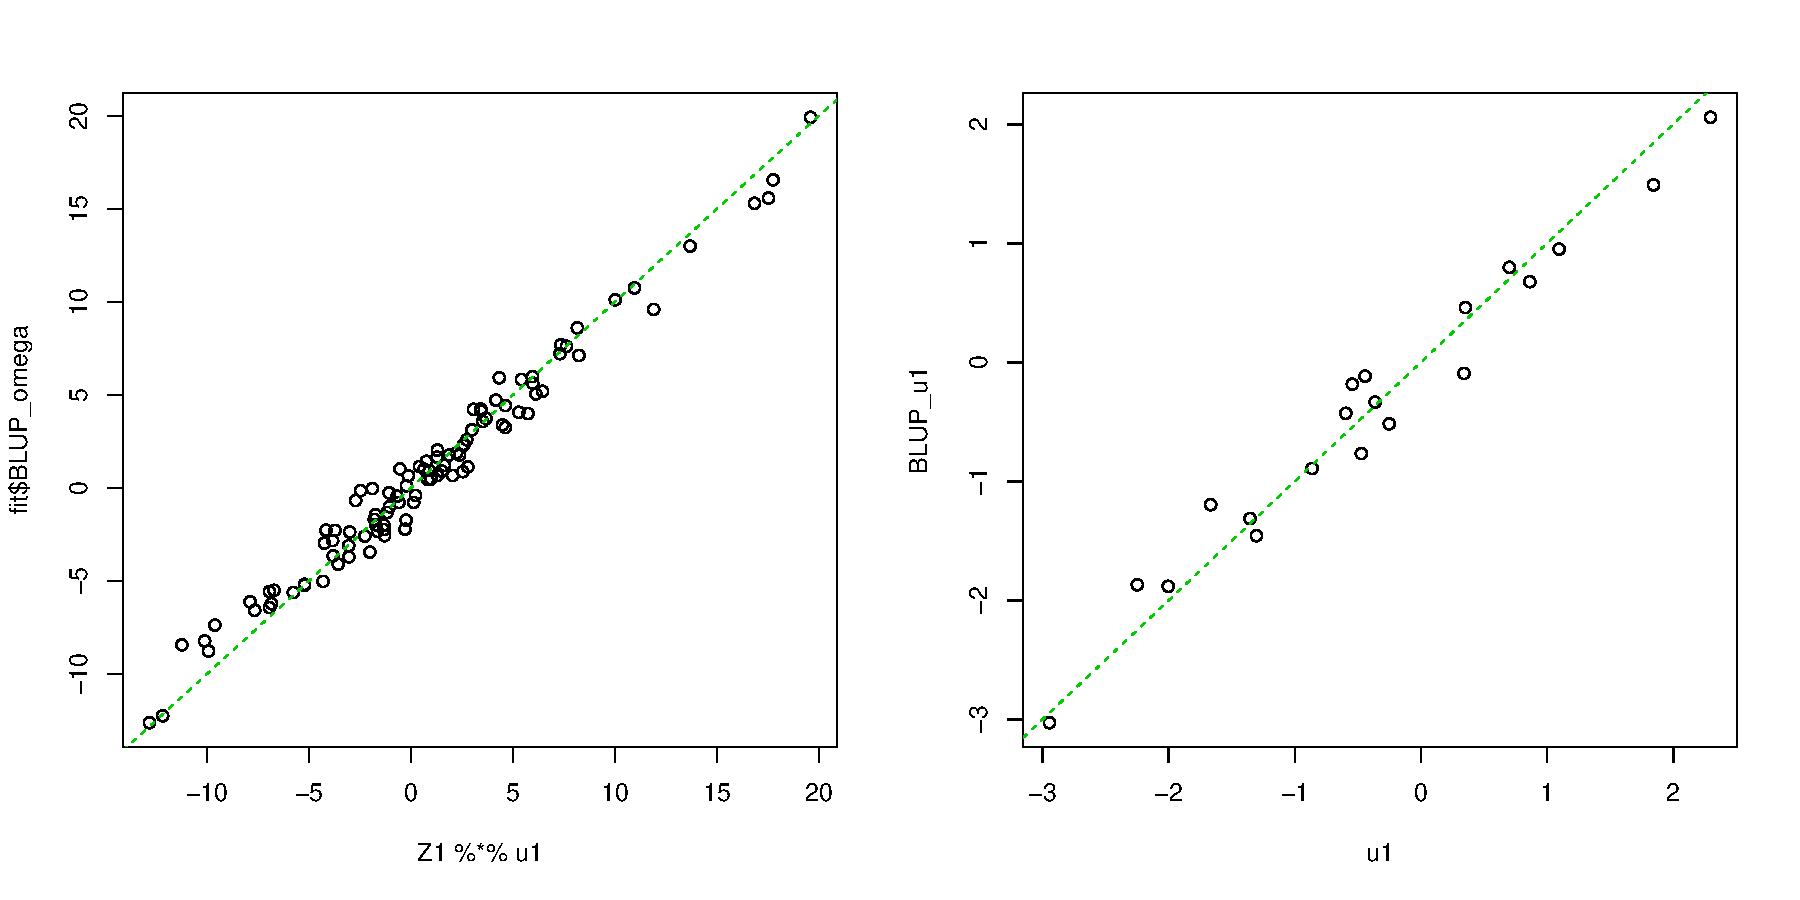
\includegraphics[width=0.7\textwidth]{figure/unnamed-chunk-40-1} 

}



\end{knitrout}
%\end{center}

  \subsubsection{Several random effects vectors}

  It is sufficient to give to \verb!lmm.aireml! a list with the two matrices
  $K_1$ and $K_2$:

\begin{knitrout}
\definecolor{shadecolor}{rgb}{0.969, 0.969, 0.969}\color{fgcolor}\begin{kframe}
\begin{alltt}
\hlstd{> }\hlstd{K2} \hlkwb{<-} \hlkwd{tcrossprod}\hlstd{(Z2)}
\hlstd{> }\hlstd{fit2} \hlkwb{<-} \hlkwd{lmm.aireml}\hlstd{(y2, X,} \hlkwc{K} \hlstd{=} \hlkwd{list}\hlstd{(K1, K2),} \hlkwc{verbose} \hlstd{=} \hlnum{FALSE}\hlstd{)}
\hlstd{> }\hlkwd{str}\hlstd{(fit2)}
\end{alltt}
\begin{verbatim}
List of 10
 $ sigma2    : num 3.04
 $ tau       : num [1:2] 1.81 0.821
 $ logL      : num -164
 $ logL0     : num -244
 $ niter     : int 13
 $ norm_grad : num 1.61e-06
 $ Py        : num [1:100] -0.353 -0.199 0.879 0.472 0.968 ...
 $ BLUP_omega: num [1:100] 0.342 -15.406 6.239 4.559 4.361 ...
 $ BLUP_beta : num [1:2] 1.1 1.98
 $ varXbeta  : num 9.33
\end{verbatim}
\end{kframe}
\end{knitrout}

  The component \verb!tau! now holds the two values $\tau_1$ and $\tau_2$.
  Note that there is only one \verb!BLUP_omega! vector. It corresponds to
  the BLUP for $\omega_1 + \omega_2$. The BLUPs for each $\omega_i$ can
  be retrieved using $\widehat{\omega_i} = \tau_i K_i Py$:

%\begin{center}
\begin{knitrout}
\definecolor{shadecolor}{rgb}{0.969, 0.969, 0.969}\color{fgcolor}\begin{kframe}
\begin{alltt}
\hlstd{> }\hlkwd{par}\hlstd{(}\hlkwc{mfrow} \hlstd{=} \hlkwd{c}\hlstd{(}\hlnum{1}\hlstd{,} \hlnum{2}\hlstd{))}
\hlstd{> }\hlstd{omega1} \hlkwb{<-} \hlstd{fit2}\hlopt{$}\hlstd{tau[}\hlnum{1}\hlstd{]} \hlopt{*} \hlstd{K1} \hlopt \hlstd{fit2}\hlopt{$}\hlstd{Py}
\hlstd{> }\hlstd{omega2} \hlkwb{<-} \hlstd{fit2}\hlopt{$}\hlstd{tau[}\hlnum{2}\hlstd{]} \hlopt{*} \hlstd{K2} \hlopt \hlstd{fit2}\hlopt{$}\hlstd{Py}
\hlstd{> }\hlkwd{plot}\hlstd{(Z1} \hlopt \hlstd{u1, omega1);} \hlkwd{abline}\hlstd{(}\hlnum{0}\hlstd{,} \hlnum{1}\hlstd{,} \hlkwc{lty} \hlstd{=} \hlnum{2}\hlstd{,} \hlkwc{col} \hlstd{=} \hlnum{3}\hlstd{)}
\hlstd{> }\hlkwd{plot}\hlstd{(Z2} \hlopt \hlstd{u2, omega2);} \hlkwd{abline}\hlstd{(}\hlnum{0}\hlstd{,} \hlnum{1}\hlstd{,} \hlkwc{lty} \hlstd{=} \hlnum{2}\hlstd{,} \hlkwc{col} \hlstd{=} \hlnum{3}\hlstd{)}
\end{alltt}
\end{kframe}

{\centering 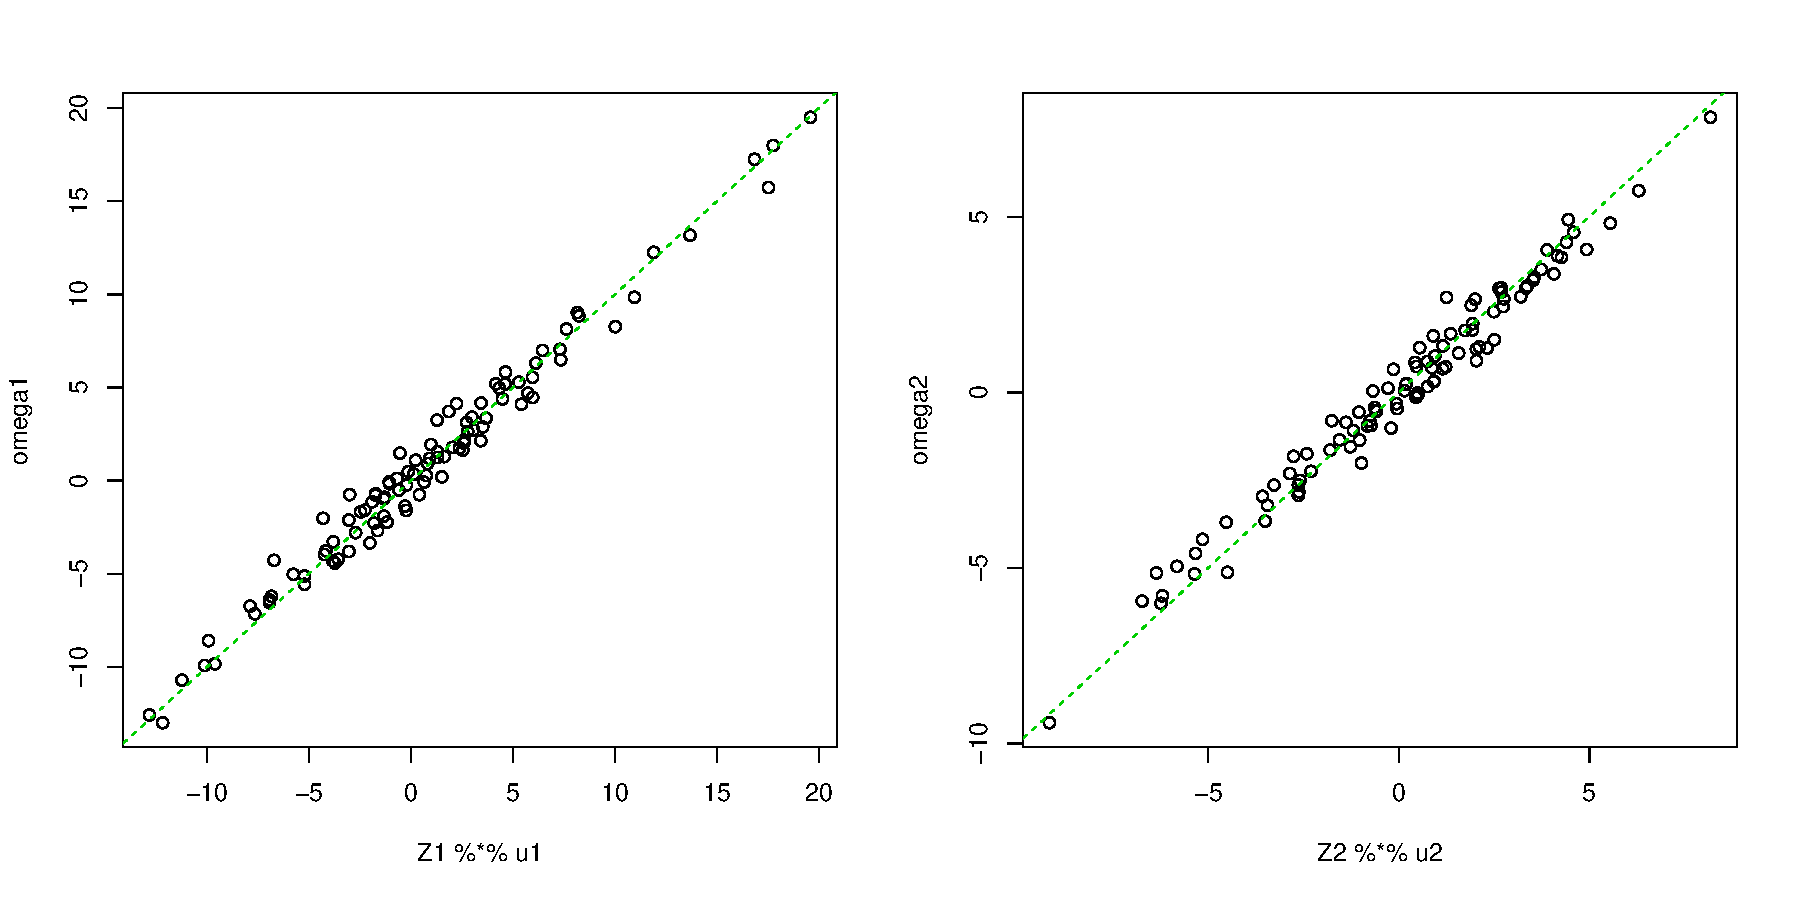
\includegraphics[width=0.7\textwidth]{figure/unnamed-chunk-42-1} 

}



\end{knitrout}
%\end{center}

  The BLUPs for $u_1$ and $u_2$ can as above be retrieved using $\widehat{u_i} = \tau_i Z_i' P y$.
  
  \subsection{Model fitting with the diagonalization trick}

  In the case where there is only one vector of random effects ($k = 1)$, the
  diagonalization trick uses the eigen decomposition of $K_1$ to speed up the 
  computation of the restricted likelihood, which allows to use a generic 
  algorithm to maximize it. Of course, the eigen decomposition of $K_1$ needs 
  to be computed beforehand, which induces an overhead. 

  The trick relies on a transformation of the data which leads to a diagonal variance matrix for $Y$. 
  The computation of a the restricted likelihood
  involves the computation of the inverse of this matrix, which is then easy to compute.
  Write the eigen decomposition of $K_1$ as $K_1 = U \Sigma^2 U'$ with $\Sigma^2$
  a diagonal matrix of positive eigenvalues, and $U$ an orthogonal matrix.
  If we let $\tilde Y = U'Y$, $\tilde X = U'X$, $\tilde \omega_1 = U' \omega_1$, and
  $\tilde\varepsilon = U' \varepsilon$, we have
  $$ \tilde Y = \tilde X\beta + \tilde \omega_1 + \tilde \varepsilon $$
  with $\tilde \omega_1 \sim N\left(0,\tau \Sigma^2\right)$ and $ \tilde\varepsilon \sim N(0,\sigma^2 I_n) $.
  As stated above, $\mathrm{var}\left(\tilde Y\right) = \tau \Sigma^2 + \sigma^2 I_n$ is diagonal.

  We fit the first model again:
 
\begin{knitrout}
\definecolor{shadecolor}{rgb}{0.969, 0.969, 0.969}\color{fgcolor}\begin{kframe}
\begin{alltt}
\hlstd{> }\hlstd{eiK1} \hlkwb{<-} \hlkwd{eigen}\hlstd{(K1)}
\hlstd{> }\hlstd{fit.d} \hlkwb{<-} \hlkwd{lmm.diago}\hlstd{(y, X, eiK1)}
\end{alltt}
\begin{verbatim}
Optimization in interval [0, 1]
Optimizing with p = 0
[Iteration 1] Current point = 0 df = 4301.78
[Iteration 2] Current point = 0.00597137 df = 2202.74
[Iteration 3] Current point = 0.0183343 df = 1073.77
[Iteration 4] Current point = 0.041009 df = 501.592
[Iteration 5] Current point = 0.0785099 df = 224.008
[Iteration 6] Current point = 0.134165 df = 94.4939
[Iteration 7] Current point = 0.206173 df = 36.1315
[Iteration 8] Current point = 0.279987 df = 10.9812
[Iteration 9] Current point = 0.326676 df = 1.82058
[Iteration 10] Current point = 0.337786 df = 0.0676512
[Iteration 11] Too many iterations, using Brent algorithm
[Iteration 11] Brent gives 0.338232
\end{verbatim}
\begin{alltt}
\hlstd{> }\hlkwd{str}\hlstd{(fit.d)}
\end{alltt}
\begin{verbatim}
List of 9
 $ sigma2    : num 3.23
 $ tau       : num 1.65
 $ Py        : num [1:100] 0.531 -0.243 0.116 0.34 -0.304 ...
 $ BLUP_omega: num [1:100] -0.443 -12.629 -1.73 5.059 5.836 ...
 $ BLUP_beta : num [1:2] 1.4 1.79
 $ varbeta   : num [1:2, 1:2] 0.134 -0.0387 -0.0387 0.016
 $ Xbeta     : num [1:100] 3.09 5.93 1.65 5.85 9.89 ...
 $ varXbeta  : num 7.51
 $ p         : int 0
\end{verbatim}
\end{kframe}
\end{knitrout}
  You can check that the result is similar to the result obtained earlier with 
  \verb!lmm.aireml!.

  The likelihood computation with the diagonalization trick is fast enough to 
  plot the likelihood:

%\setkeys{Gin}{width=0.4\textwidth}
%\begin{center}
\begin{knitrout}
\definecolor{shadecolor}{rgb}{0.969, 0.969, 0.969}\color{fgcolor}\begin{kframe}
\begin{alltt}
\hlstd{> }\hlstd{TAU} \hlkwb{<-} \hlkwd{seq}\hlstd{(}\hlnum{0.5}\hlstd{,}\hlnum{2.5}\hlstd{,}\hlkwc{length}\hlstd{=}\hlnum{50}\hlstd{)}
\hlstd{> }\hlstd{S2} \hlkwb{<-} \hlkwd{seq}\hlstd{(}\hlnum{2.5}\hlstd{,}\hlnum{4}\hlstd{,}\hlkwc{length}\hlstd{=}\hlnum{50}\hlstd{)}
\hlstd{> }\hlstd{lik} \hlkwb{<-} \hlkwd{lmm.diago.likelihood}\hlstd{(}\hlkwc{tau} \hlstd{= TAU,} \hlkwc{s2} \hlstd{= S2,} \hlkwc{Y} \hlstd{= y,} \hlkwc{X} \hlstd{= X,} \hlkwc{eigenK} \hlstd{= eiK1)}
\hlstd{> }\hlkwd{lik.contour}\hlstd{(TAU, S2, lik,} \hlkwc{heat} \hlstd{=} \hlnum{TRUE}\hlstd{,} \hlkwc{xlab} \hlstd{=} \hlstr{"tau"}\hlstd{,} \hlkwc{ylab} \hlstd{=} \hlstr{"sigma^2"}\hlstd{)}
\end{alltt}
\end{kframe}

{\centering 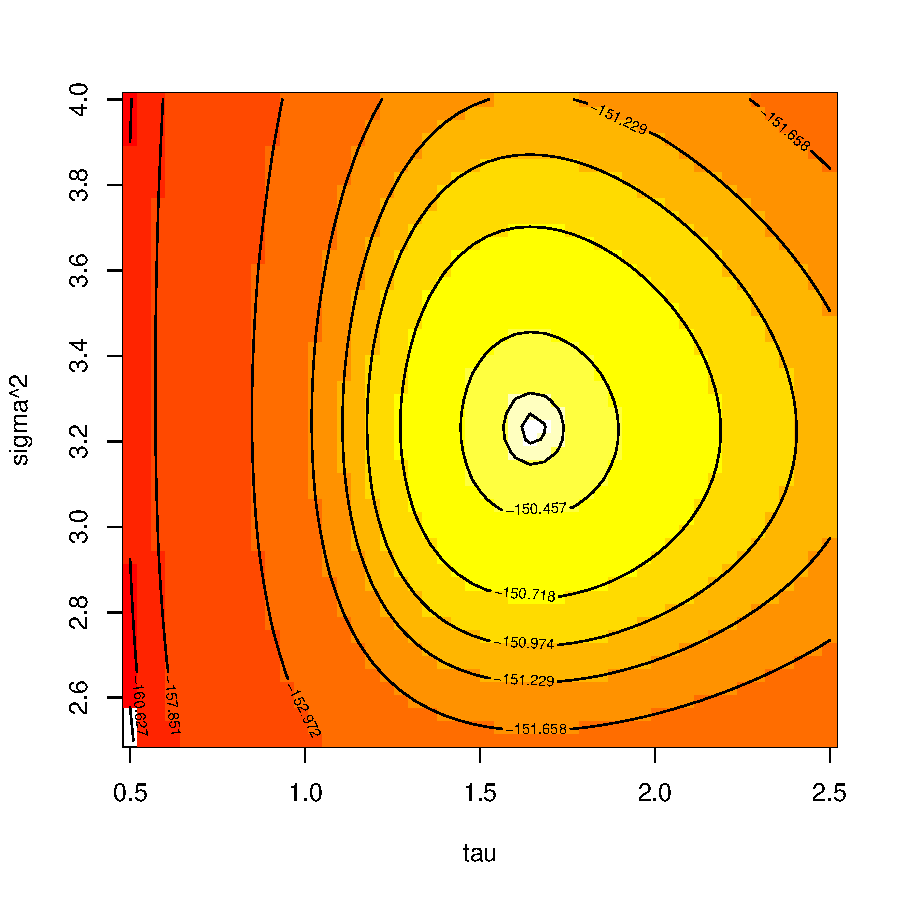
\includegraphics[width=0.4\textwidth]{figure/unnamed-chunk-44-1} 

}



\end{knitrout}
%\end{center}



\subsection{Genomic heritability estimation with Gaston}

  Heritability estimates based on Genetic Relationship Matrices (GRM)
  are computed under the following model:
  \begin{equation*}
  Y = \beta + \omega + \epsilon
  \end{equation*}
  where $\omega \sim \N(0, \tau K)$ and $\epsilon\sim \N(0, \sigma^2 I_n)$,
  $K$ being a GRM computed on whole genome data (e.g. by the function \verb!GRM!).
  The heritability is $h^2 = {\tau \over \tau + \sigma^2}$.

  Note that as $K = {1\over q-1} X_sX_s'$ with $X_s$ a standardized genotype matrix, 
  letting $Z = (q-1)^{-{1 \over 2}} X_s$, this model is equivalent to 
  \begin{equation*}
  Y = \beta + Zu + \epsilon
  \end{equation*}
  with $u \sim \N(0,\tau I_q)$.

  The function \verb!random.pm! generates random positive matrices with eigenvalues
  roughly similar to those typically observed when using whole genome data. It outputs a list
  with a member \verb!K!: a positive matrix, and a member \verb!eigen!: its eigen 
  decomposition (as the base function \verb!eigen! would output it).

  The function \verb!lmm.simu! can be used simulate data under the linear mixed model.
  It uses the eigen decomposition of $K$. Hereafter we use $\tau = 1$, $\sigma^2 = 2$,
  hence a $33.3\%$ heritability.

\begin{knitrout}
\definecolor{shadecolor}{rgb}{0.969, 0.969, 0.969}\color{fgcolor}\begin{kframe}
\begin{alltt}
\hlstd{> }\hlkwd{set.seed}\hlstd{(}\hlnum{1}\hlstd{)}
\hlstd{> }\hlstd{n} \hlkwb{<-} \hlnum{2000}
\hlstd{> }\hlstd{R} \hlkwb{<-} \hlkwd{random.pm}\hlstd{(n)}
\hlstd{> }\hlstd{y} \hlkwb{<-} \hlnum{2} \hlopt{+} \hlkwd{lmm.simu}\hlstd{(}\hlkwc{tau} \hlstd{=} \hlnum{1}\hlstd{,} \hlkwc{sigma2} \hlstd{=} \hlnum{2}\hlstd{,} \hlkwc{eigenK} \hlstd{= R}\hlopt{$}\hlstd{eigen)}\hlopt{$}\hlstd{y}
\end{alltt}
\end{kframe}
\end{knitrout}

  We can use \verb!lmm.diago! to estimates the parameters of the model.

\begin{knitrout}
\definecolor{shadecolor}{rgb}{0.969, 0.969, 0.969}\color{fgcolor}\begin{kframe}
\begin{alltt}
\hlstd{> }\hlstd{fit} \hlkwb{<-} \hlkwd{lmm.diago}\hlstd{(y,} \hlkwc{eigenK} \hlstd{= R}\hlopt{$}\hlstd{eigen)}
\end{alltt}
\begin{verbatim}
Optimization in interval [0, 1]
Optimizing with p = 0
[Iteration 1] Current point = 0 df = 3.32616
[Iteration 2] Current point = 0.099573 df = 0.0543536
[Iteration 3] Current point = 0.101252 df = 1.2657e-05
\end{verbatim}
\end{kframe}
\end{knitrout}


  We have $\widehat\tau = 0.298$ and $\widehat{\sigma^2} = 2.65$,
  hence $h^2$ is estimated to $10.1\%$.

  The function \verb!lmm.diago.likelihood! allows to compute a profile likelihood with parameter 
  $h^2 = {\tau \over \tau + \sigma^2}$. It can be useful to get confidence intervals. Here,
  we simply plot it:

%\begin{center}
\begin{knitrout}
\definecolor{shadecolor}{rgb}{0.969, 0.969, 0.969}\color{fgcolor}\begin{kframe}
\begin{alltt}
\hlstd{> }\hlstd{H2} \hlkwb{<-} \hlkwd{seq}\hlstd{(}\hlnum{0}\hlstd{,}\hlnum{1}\hlstd{,}\hlkwc{length}\hlstd{=}\hlnum{51}\hlstd{)}
\hlstd{> }\hlstd{lik} \hlkwb{<-} \hlkwd{lmm.diago.likelihood}\hlstd{(}\hlkwc{h2} \hlstd{= H2,} \hlkwc{Y} \hlstd{= y,} \hlkwc{eigenK} \hlstd{= R}\hlopt{$}\hlstd{eigen)}
\hlstd{> }\hlkwd{plot}\hlstd{(H2,} \hlkwd{exp}\hlstd{(lik}\hlopt{$}\hlstd{likelihood}\hlopt{-}\hlkwd{max}\hlstd{(lik}\hlopt{$}\hlstd{likelihood)),} \hlkwc{type}\hlstd{=}\hlstr{"l"}\hlstd{,} \hlkwc{yaxt}\hlstd{=}\hlstr{"n"}\hlstd{,} \hlkwc{ylab}\hlstd{=}\hlstr{"likelihood"}\hlstd{)}
\end{alltt}
\end{kframe}

{\centering 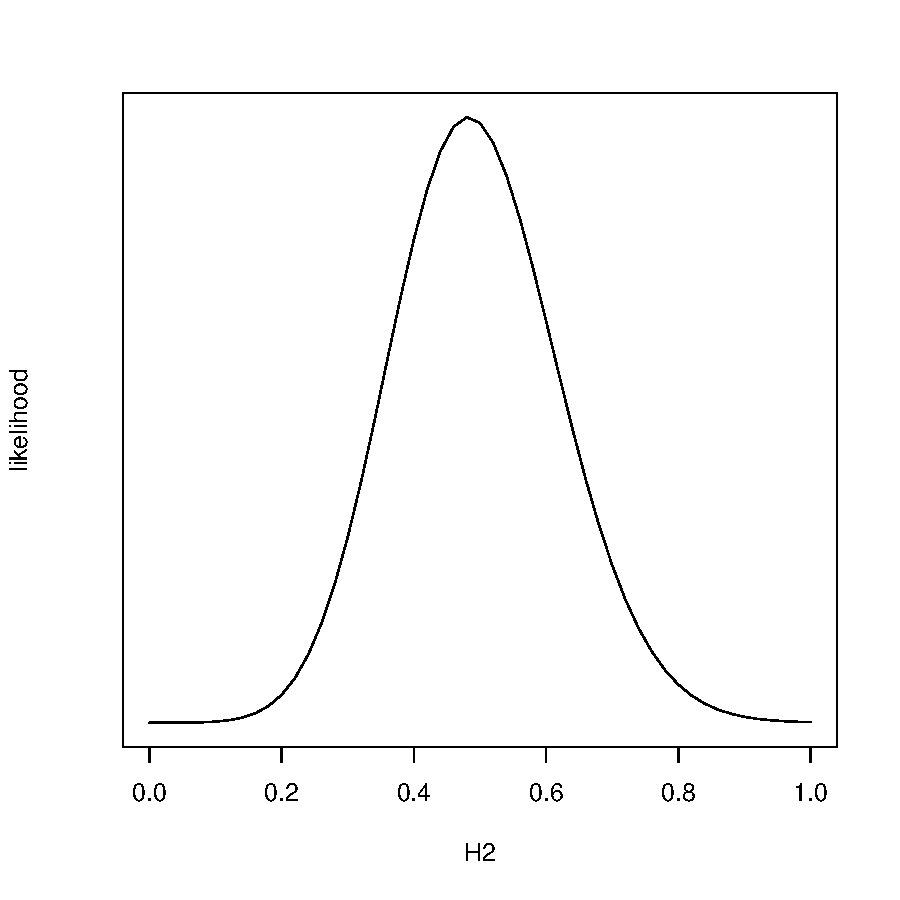
\includegraphics[width=0.4\textwidth]{figure/unnamed-chunk-48-1} 

}



\end{knitrout}
%\end{center}

  It is often advised to include the first few (10 or 20) Principal Components (PC) in the model as fixed effects,
  to account for a possible population stratification. The function \verb!lmm.diago! has an argument \verb!p!
  for the number of PCs to incoporate in the model with fixed effects. We simulate a trait with a large effect of
  the two first PCs:
\begin{knitrout}
\definecolor{shadecolor}{rgb}{0.969, 0.969, 0.969}\color{fgcolor}\begin{kframe}
\begin{alltt}
\hlstd{> }\hlstd{PC} \hlkwb{<-} \hlkwd{sweep}\hlstd{(R}\hlopt{$}\hlstd{eigen}\hlopt{$}\hlstd{vectors,} \hlnum{2}\hlstd{,} \hlkwd{sqrt}\hlstd{(R}\hlopt{$}\hlstd{eigen}\hlopt{$}\hlstd{values),} \hlstr{"*"}\hlstd{)}
\hlstd{> }\hlstd{y1} \hlkwb{<-} \hlnum{2} \hlopt{+} \hlstd{PC[,}\hlnum{1}\hlopt{:}\hlnum{2}\hlstd{]} \hlopt \hlkwd{c}\hlstd{(}\hlnum{5}\hlstd{,}\hlnum{5}\hlstd{)} \hlopt{+} \hlkwd{lmm.simu}\hlstd{(}\hlkwc{tau} \hlstd{=} \hlnum{1}\hlstd{,} \hlkwc{sigma2} \hlstd{=} \hlnum{2}\hlstd{,} \hlkwc{eigenK} \hlstd{= R}\hlopt{$}\hlstd{eigen)}\hlopt{$}\hlstd{y}
\end{alltt}
\end{kframe}
\end{knitrout}

  Here are the heritability estimates with $p = 0$ (the default) and $p = 10$.
\begin{knitrout}
\definecolor{shadecolor}{rgb}{0.969, 0.969, 0.969}\color{fgcolor}\begin{kframe}
\begin{alltt}
\hlstd{> }\hlstd{fit0} \hlkwb{<-} \hlkwd{lmm.diago}\hlstd{(y1,} \hlkwc{eigenK} \hlstd{= R}\hlopt{$}\hlstd{eigen)}
\end{alltt}
\begin{verbatim}
Optimization in interval [0, 1]
Optimizing with p = 0
[Iteration 1] Current point = 0 df = 8.47139
[Iteration 2] Current point = 0.239713 df = 0.364915
[Iteration 3] Current point = 0.2509 df = 0.000461187
[Iteration 4] Current point = 0.250914 df = 7.18119e-10
\end{verbatim}
\begin{alltt}
\hlstd{> }\hlstd{fit0}\hlopt{$}\hlstd{tau}\hlopt{/}\hlstd{(fit0}\hlopt{$}\hlstd{tau}\hlopt{+}\hlstd{fit0}\hlopt{$}\hlstd{sigma2)}
\end{alltt}
\begin{verbatim}
[1] 0.2509142
\end{verbatim}
\begin{alltt}
\hlstd{> }\hlstd{fit10} \hlkwb{<-} \hlkwd{lmm.diago}\hlstd{(y1,} \hlkwc{eigenK} \hlstd{= R}\hlopt{$}\hlstd{eigen,} \hlkwc{p} \hlstd{=} \hlnum{10}\hlstd{)}
\end{alltt}
\begin{verbatim}
Optimization in interval [0, 1]
Optimizing with p = 10
[Iteration 1] Current point = 0 df = 4.45003
[Iteration 2] Current point = 0.143356 df = 0.0854252
[Iteration 3] Current point = 0.146209 df = 2.38332e-05
\end{verbatim}
\begin{alltt}
\hlstd{> }\hlstd{fit10}\hlopt{$}\hlstd{tau}\hlopt{/}\hlstd{(fit10}\hlopt{$}\hlstd{tau}\hlopt{+}\hlstd{fit10}\hlopt{$}\hlstd{sigma2)}
\end{alltt}
\begin{verbatim}
[1] 0.1462102
\end{verbatim}
\end{kframe}
\end{knitrout}

  As expected, the estimate is inflated when no PCs are incorporated in the model.
 
%%%%%%%%%%%%%%%%%%%%%%%%%%%%%%%%%%%%%%%%%%%%%%%%%%%%%%%%%%%%%%%%%%%%%%%%%%%%%%%%%%%%%%%%%%%%%%%%%%%%
\vfill\eject
\section{Association test}

The function described here is rapidly evolving, and this description is incomplete. 
Stay tuned!

\subsection{Quantitative trait}

  The function \verb!association.test! performs a test of association between SNPs 
  and a quantitative trait $Y$ under the following model
\begin{equation*}
  Y = (X|PC)\alpha + G\beta + \omega + \varepsilon 
\end{equation*}
  where $X$ is the matrix of covariables with fixed effects (including a column 
  of ones for the intercept), $G$ is the vector of genotypes at the SNP under
  consideration, and $\omega\sim\N(0,\tau K)$ where $K$ is a Genetic Relationship
  Matrix (computed on the whole genome). A few PCs can be included in the model
  with fixed effects (using parameter \verb!p! as above for \verb!lmm.diago!).

  Three tests are proposed for $H_0: \beta = 0$: a score test, a Wald test on $\widehat\beta$,
  or a Likelihood Ratio Test.

  We illustrate this function on a simple example, built on the AGT data set:
\begin{knitrout}
\definecolor{shadecolor}{rgb}{0.969, 0.969, 0.969}\color{fgcolor}\begin{kframe}
\begin{alltt}
\hlstd{> }\hlkwd{data}\hlstd{(AGT)}
\hlstd{> }\hlstd{x} \hlkwb{<-} \hlkwd{as.bed.matrix}\hlstd{(AGT.gen, AGT.fam, AGT.bim)}
\hlstd{> }\hlkwd{standardize}\hlstd{(x)} \hlkwb{<-} \hlstr{'mu'}
\end{alltt}
\end{kframe}
\end{knitrout}

  As the whole genome is not available, we generate a random positive matrix to play the role of the GRM:
\begin{knitrout}
\definecolor{shadecolor}{rgb}{0.969, 0.969, 0.969}\color{fgcolor}\begin{kframe}
\begin{alltt}
\hlstd{> }\hlkwd{set.seed}\hlstd{(}\hlnum{1}\hlstd{)}
\hlstd{> }\hlstd{R} \hlkwb{<-} \hlkwd{random.pm}\hlstd{(}\hlkwd{nrow}\hlstd{(x))}
\end{alltt}
\end{kframe}
\end{knitrout}

  And we simulate a phenotype with an effect of the SNP \#351, and a polygenic component:
\begin{knitrout}
\definecolor{shadecolor}{rgb}{0.969, 0.969, 0.969}\color{fgcolor}\begin{kframe}
\begin{alltt}
\hlstd{> }\hlstd{y} \hlkwb{<-} \hlnum{2} \hlopt{+} \hlstd{x} \hlopt \hlkwd{c}\hlstd{(}\hlkwd{rep}\hlstd{(}\hlnum{0}\hlstd{,}\hlnum{350}\hlstd{),}\hlnum{0.25}\hlstd{,}\hlkwd{rep}\hlstd{(}\hlnum{0}\hlstd{,}\hlkwd{ncol}\hlstd{(x)}\hlopt{-}\hlnum{351}\hlstd{))} \hlopt{+}
\hlstd{+ }     \hlkwd{lmm.simu}\hlstd{(}\hlkwc{tau} \hlstd{=} \hlnum{0.3}\hlstd{,} \hlkwc{sigma2} \hlstd{=} \hlnum{1}\hlstd{,} \hlkwc{eigenK}\hlstd{=R}\hlopt{$}\hlstd{eigen)}\hlopt{$}\hlstd{y}
\end{alltt}
\end{kframe}
\end{knitrout}

  The following code performs the association test with a score test and a wald test,
  and compares the resulting $p$-values:
%\begin{center}
\begin{knitrout}
\definecolor{shadecolor}{rgb}{0.969, 0.969, 0.969}\color{fgcolor}\begin{kframe}
\begin{alltt}
\hlstd{> }\hlstd{t_score} \hlkwb{<-} \hlkwd{association.test}\hlstd{(x, y,} \hlkwc{K} \hlstd{= R}\hlopt{$}\hlstd{K,} \hlkwc{method} \hlstd{=} \hlstr{"lmm"}\hlstd{)}
\end{alltt}
\begin{verbatim}
[Iteration 1] theta = 0.708172 0.708172
[Iteration 1] log L = -342.103
[Iteration 1] Constraining tau
[Iteration 1] AI-REML update
[Iteration 1] ||gradient|| = 1.20936
[Iteration 2] theta = 1.41153   1e-06
[Iteration 2] log L = -341.48
[Iteration 2] AI-REML update
[Iteration 2] ||gradient|| = 0.606817
[Iteration 3] theta = 1.41633   1e-06
[Iteration 3] log L = -341.478
[Iteration 3] AI-REML update
[Iteration 3] ||gradient|| = 0.00204975
[Iteration 4] theta = 1.41634   1e-06
[Iteration 4] log L = -341.478
[Iteration 4] Checking gradient components signs before last iteration
[Iteration 4] AI-REML update
[Iteration 4] ||gradient|| = 2.37022e-08
\end{verbatim}
\begin{alltt}
\hlstd{> }\hlstd{t_wald} \hlkwb{<-} \hlkwd{association.test}\hlstd{(x, y,} \hlkwc{eigenK} \hlstd{= R}\hlopt{$}\hlstd{eigen,} \hlkwc{method} \hlstd{=} \hlstr{"lmm"}\hlstd{,} \hlkwc{test} \hlstd{=} \hlstr{"wald"}\hlstd{)}
\hlstd{> }\hlkwd{plot}\hlstd{( t_score}\hlopt{$}\hlstd{p, t_wald}\hlopt{$}\hlstd{p,} \hlkwc{log} \hlstd{=} \hlstr{"xy"}\hlstd{,} \hlkwc{xlab} \hlstd{=} \hlstr{"score"}\hlstd{,} \hlkwc{ylab} \hlstd{=} \hlstr{"wald"}\hlstd{)}
\end{alltt}
\end{kframe}

{\centering 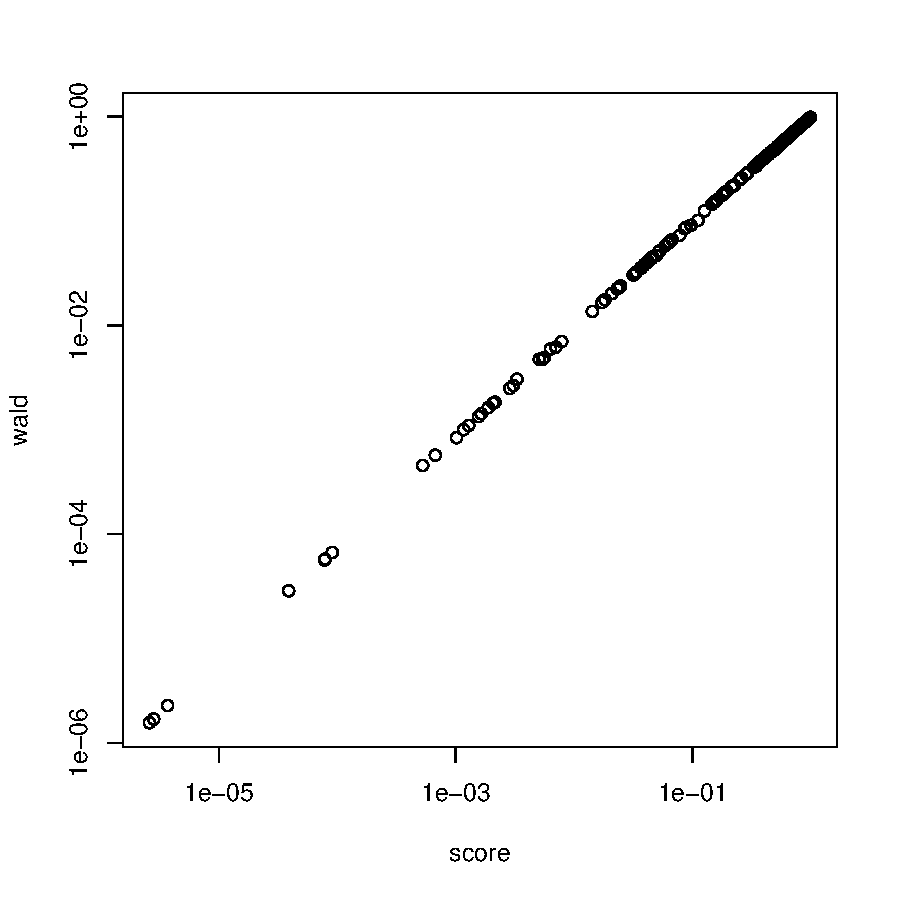
\includegraphics[width=0.4\textwidth]{figure/unnamed-chunk-54-1} 

}



\end{knitrout}
%\end{center}

We can display the results under the form of a (mini) Manhattan plot:
%\begin{center}
%\setkeys{Gin}{width=0.7\textwidth}
\begin{knitrout}
\definecolor{shadecolor}{rgb}{0.969, 0.969, 0.969}\color{fgcolor}\begin{kframe}
\begin{alltt}
\hlstd{> }\hlkwd{plot}\hlstd{(}\hlopt{-}\hlkwd{log10}\hlstd{(t_score}\hlopt{$}\hlstd{p),} \hlkwc{xlab}\hlstd{=}\hlstr{"SNP index"}\hlstd{,} \hlkwc{ylab} \hlstd{=} \hlstr{"-log(p)"}\hlstd{,}
\hlstd{+ }      \hlkwc{col} \hlstd{=} \hlkwd{c}\hlstd{(}\hlkwd{rep}\hlstd{(}\hlnum{1}\hlstd{,}\hlnum{350}\hlstd{),}\hlnum{2}\hlstd{,}\hlkwd{rep}\hlstd{(}\hlnum{1}\hlstd{,}\hlkwd{ncol}\hlstd{(x)}\hlopt{-}\hlnum{351}\hlstd{)))}
\end{alltt}
\end{kframe}

{\centering 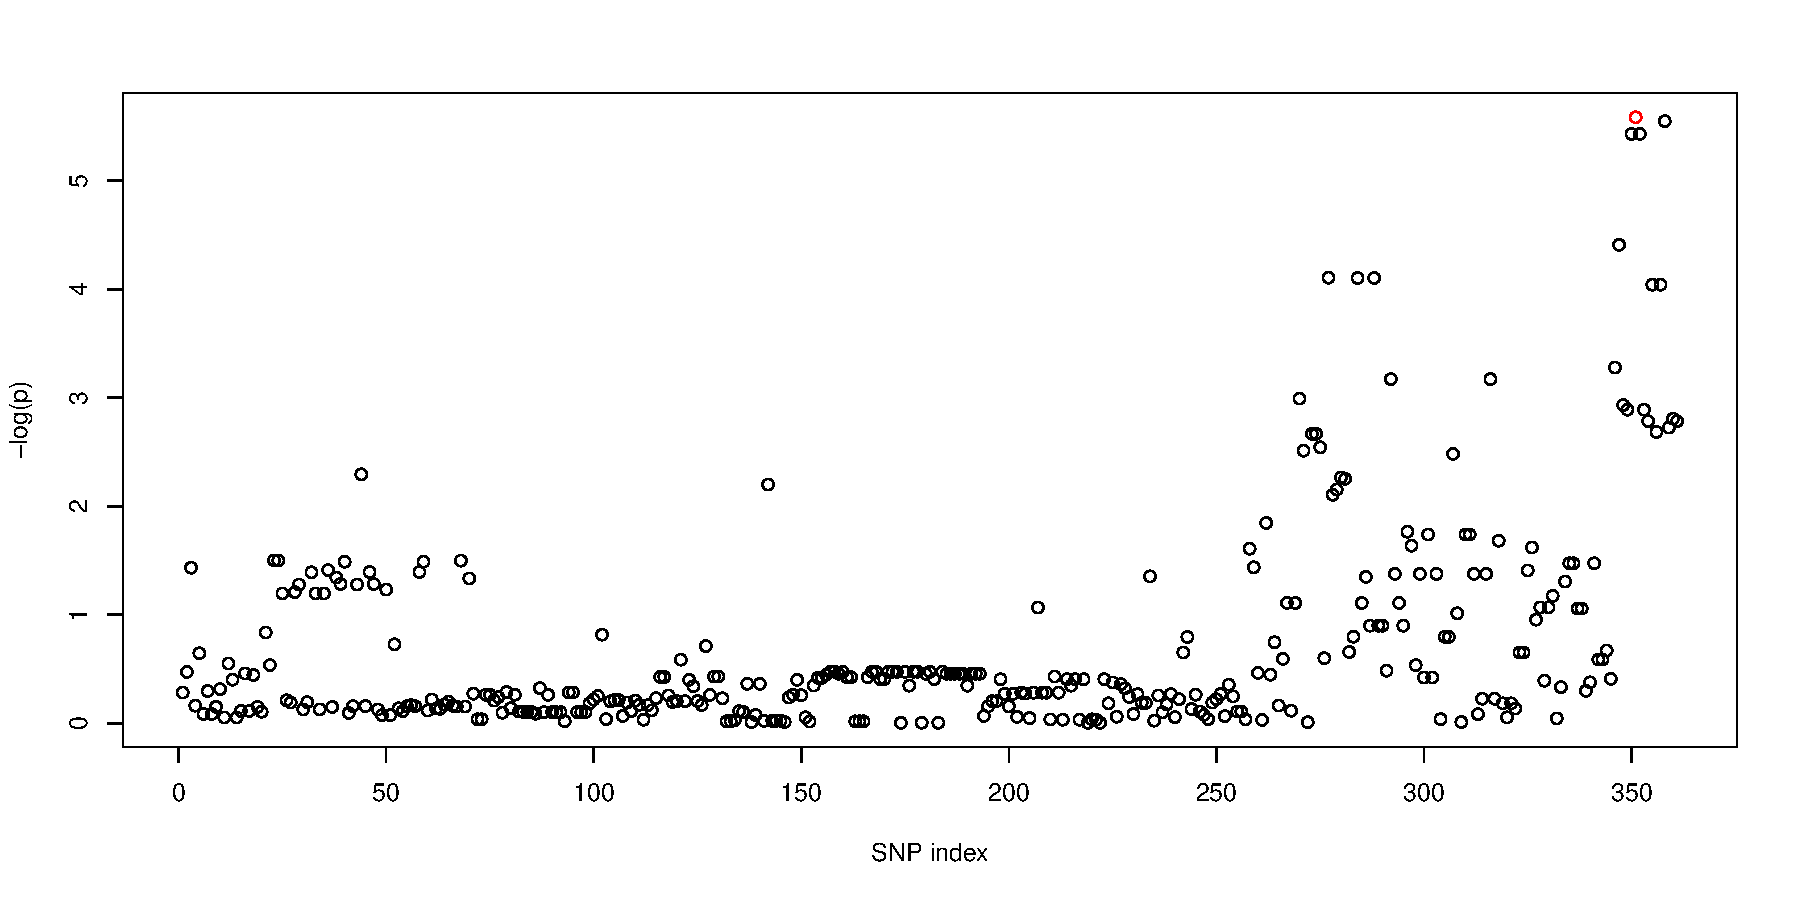
\includegraphics[width=0.7\textwidth]{figure/unnamed-chunk-55-1} 

}



\end{knitrout}
%\end{center}

  We colored the point corresponding to the SNP \#351 in red. We see that there
  are other SNPs with low association $p$-values: these are the SNPs in LD with
  SNP \#351. We can confirm this by plotting the $p$-values (again on log scale) 
  as a function of the LD (measured by $r^2$):
%\begin{center}
\begin{knitrout}
\definecolor{shadecolor}{rgb}{0.969, 0.969, 0.969}\color{fgcolor}\begin{kframe}
\begin{alltt}
\hlstd{> }\hlstd{lds} \hlkwb{<-} \hlkwd{LD}\hlstd{(x,} \hlnum{351}\hlstd{,} \hlkwd{c}\hlstd{(}\hlnum{1}\hlstd{,}\hlkwd{ncol}\hlstd{(x)))}
\hlstd{> }\hlkwd{plot}\hlstd{(lds,} \hlopt{-}\hlkwd{log10}\hlstd{(t_score}\hlopt{$}\hlstd{p),} \hlkwc{xlab}\hlstd{=}\hlstr{"r^2"}\hlstd{,} \hlkwc{ylab}\hlstd{=}\hlstr{"-log(p)"}\hlstd{)}
\end{alltt}
\end{kframe}

{\centering 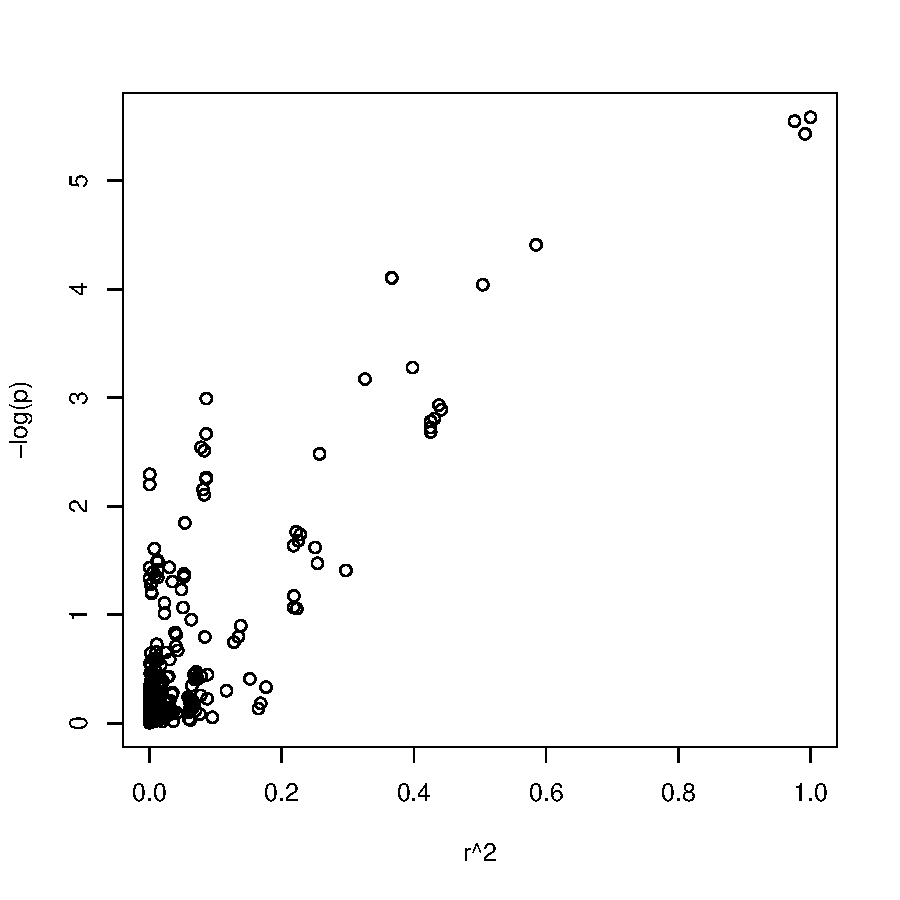
\includegraphics[width=0.4\textwidth]{figure/unnamed-chunk-56-1} 

}



\end{knitrout}
%\end{center}

\subsection{Binary phenotype}

We use the quantitative phenotype previously generated to construct a binary phenotype,
and we perform the association test with a logistic mixed model (only the score test is 
available). The baby Manhattan plot is plotted again.
%\begin{center}
%\setkeys{Gin}{width=0.7\textwidth}
\begin{knitrout}
\definecolor{shadecolor}{rgb}{0.969, 0.969, 0.969}\color{fgcolor}\begin{kframe}
\begin{alltt}
\hlstd{> }\hlstd{y1} \hlkwb{<-} \hlkwd{as.numeric}\hlstd{(y} \hlopt{>} \hlkwd{mean}\hlstd{(y))}
\hlstd{> }\hlstd{t_binary} \hlkwb{<-} \hlkwd{association.test}\hlstd{(x, y1,} \hlkwc{K} \hlstd{= R}\hlopt{$}\hlstd{K,} \hlkwc{method} \hlstd{=} \hlstr{"lmm"}\hlstd{,} \hlkwc{response} \hlstd{=} \hlstr{"binary"}\hlstd{)}
\end{alltt}
\begin{verbatim}
[Initialization] beta = -0.0198814
[Initialization] tau = 4.00836
[Iteration 1] tau = 3.01058
[Iteration 1] beta = -0.0187091
[Iteration 2] gr = -11.4953
[Iteration 2] Constraining tau
[Iteration 2] tau = 1e-06
[Iteration 2] beta = -0.022655
[Iteration 3] gr = 0.0757621
[Iteration 3] tau = 0.00479595
[Iteration 3] beta = -0.0198767
[Iteration 4] gr = -0.00152393
[Iteration 4] tau = 0.00469915
[Iteration 4] beta = -0.0198768
[Iteration 5] gr = -6.65199e-06
[Iteration 5] tau = 0.00469873
[Iteration 5] beta = -0.0198768
[Iteration 6] gr = -2.47279e-08
[Iteration 6] tau = 0.00469873
[Iteration 6] beta = -0.0198768
\end{verbatim}
\begin{alltt}
\hlstd{> }\hlcom{# (mini) Manhattan plot}
\hlstd{> }\hlkwd{plot}\hlstd{(}\hlopt{-}\hlkwd{log10}\hlstd{(t_binary}\hlopt{$}\hlstd{p),} \hlkwc{xlab}\hlstd{=}\hlstr{"SNP index"}\hlstd{,} \hlkwc{ylab} \hlstd{=} \hlstr{"-log(p)"}\hlstd{,}
\hlstd{+ }      \hlkwc{col} \hlstd{=} \hlkwd{c}\hlstd{(}\hlkwd{rep}\hlstd{(}\hlnum{1}\hlstd{,}\hlnum{350}\hlstd{),}\hlnum{2}\hlstd{,}\hlkwd{rep}\hlstd{(}\hlnum{1}\hlstd{,}\hlkwd{ncol}\hlstd{(x)}\hlopt{-}\hlnum{351}\hlstd{)))}
\end{alltt}
\end{kframe}

{\centering 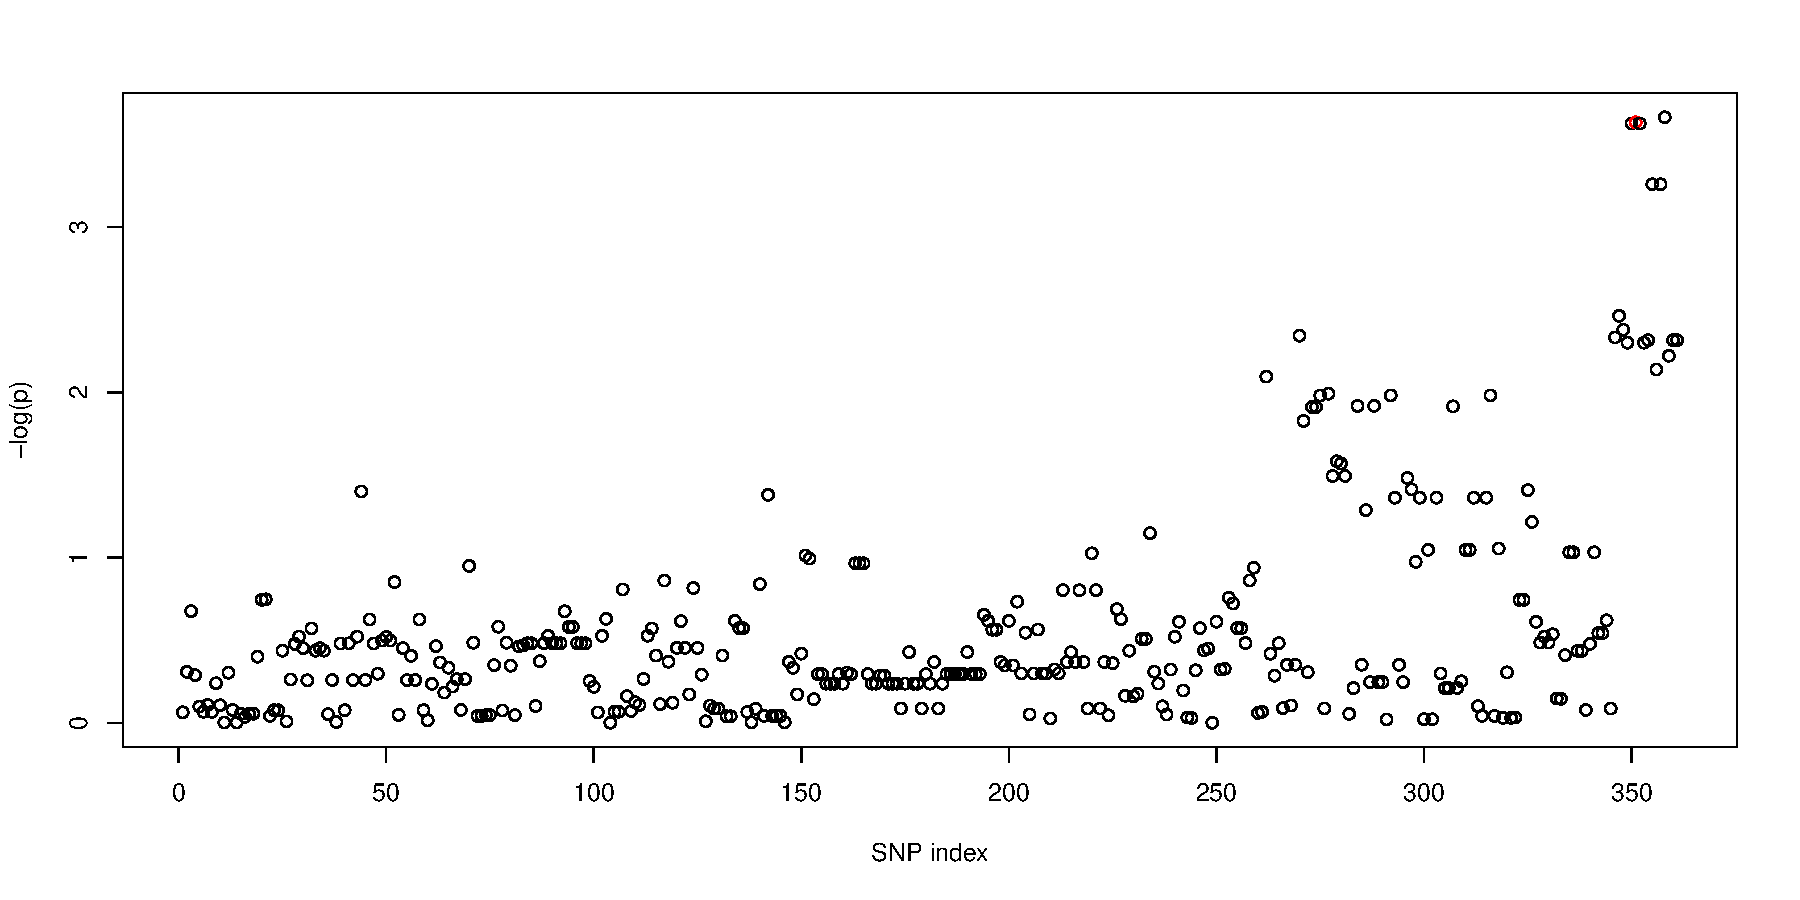
\includegraphics[width=0.7\textwidth]{figure/unnamed-chunk-57-1} 

}



\end{knitrout}
%\end{center}

%%%%%%%%%%%%%%%%%%%%%%%%%%%%%%%%%%%%%%%%%%%%%%%%%%%%%%%%%%%%%%%%%%%%%%%%%%%%%%%%%%%%%%%%%%%%%%%%%%%%
\vfill\eject
\section{What you can hope for in later releases}

A few things that may be added to the package in the near future:

\begin{itemize}
\item Reading \verb!.ped! files
\item Maximum Likelihood Linkage Disequilibrium estimation
\item LMM models fitting written in equation form
\item A faster version of \verb!association.test!
\item More functions and models for association testing
\item Anything you asked the maintainer for
\end{itemize}

\end{document}




